%% Copyright 2012-2013 by abnTeX2 group at http://abntex2.googlecode.com/ 
%%
%% This work may be distributed and/or modified under the
%% conditions of the LaTeX Project Public License, either version 1.3
%% of this license or (at your option) any later version.
%% The latest version of this license is in
%%   http://www.latex-project.org/lppl.txt
%% and version 1.3 or later is part of all distributions of LaTeX
%% version 2005/12/01 or later.
%%
%% This work has the LPPL maintenance status `maintained'.
%% 
%% The Current Maintainer of this work is the abnTeX2 team, led
%% by Lauro César Araujo. Further information are available on 
%% http://abntex2.googlecode.com/
%%
\documentclass[
	% -- opções da classe memoir --
	12pt,				% tamanho da fonte
	openright,			% capítulos começam em pág ímpar (insere página vazia caso preciso)
	oneside,				% para impressão em verso e anverso. Oposto a oneside
	a4paper,				% tamanho do papel. 
	% -- opções da classe abntex2 --
	%chapter=TITLE,			% títulos de capítulos convertidos em letras maiúsculas
	%section=TITLE,			% títulos de seções convertidos em letras maiúsculas
	%subsection=TITLE,		% títulos de subseções convertidos em letras maiúsculas
	%subsubsection=TITLE,		% títulos de subsubseções convertidos em letras maiúsculas
	% -- opções do pacote babel --
	english,				% idioma adicional para hifenização
	french,				% idioma adicional para hifenização
	spanish,				% idioma adicional para hifenização
	brazil,				% o último idioma é o principal do documento
	]{abntex2}

% ---
% Pacotes fundamentais 
% ---
\usepackage{cmap}			% Mapear caracteres especiais no PDF
\usepackage{lmodern}			% Usa a fonte Latin Modern			
\usepackage[T1]{fontenc}			% Selecao de codigos de fonte.
\usepackage[utf8]{inputenc}		% Codificacao do documento (conversão automática dos acentos)
\usepackage{lastpage}			% Usado pela Ficha catalográfica
\usepackage{indentfirst}			% Indenta o primeiro parágrafo de cada seção.
\usepackage{color}			% Controle das cores
\usepackage{graphicx}			% Inclusão de gráficos
\usepackage{listings}			% Códigos
\usepackage{xcolor}			% Pacote de cores
% ---
		
% ---
% Pacotes de citações
% ---
\usepackage[brazilian,hyperpageref]{backref}	 % Paginas com as citações na bibl
% Se o pacote brazilian não estiver instalado
%\usepackage[hyperpageref]{backref}
\usepackage[num]{abntex2cite}	% Citações padrão ABNT (alf ou num)

% --- 
% CONFIGURAÇÕES DE PACOTES
% ---
% Usar com o pacote brazilian do backref
% Configurações do pacote backref
% Usado sem a opção hyperpageref de backref
\renewcommand{\backrefpagesname}{Citado na(s) página(s):~}
% Texto padrão antes do número das páginas
\renewcommand{\backref}{}
% Define os textos da citação
\renewcommand*{\backrefalt}[4]{
	\ifcase #1 %
		Nenhuma citação no texto.%
	\or
		Citado na página #2.%
	\else
		Citado #1 vezes nas páginas #2.%
	\fi}%

% Remove os espaços na lista de figuras e tabelas
\newcommand*{\noaddvspace}{\renewcommand*{\addvspace}[1]{}}
\addtocontents{lof}{\protect\noaddvspace}
\addtocontents{lot}{\protect\noaddvspace}

% Define listing style
\definecolor{mygreen}{RGB}{0,120,0}
\definecolor{myblue}{RGB}{0,0,163}
\renewcommand{\lstlistingname}{Código}

% Custom XML/RDF style
\lstdefinestyle{customBash}{
  language=Bash,
  basicstyle=\tiny,  
  backgroundcolor=\color{white},
  breaklines=true,
  captionpos=b,  
  commentstyle=\color{gray},  
  morekeywords={bundle, gem, rake, rails, new, generate, create, install, build, sudo},
  frame=single,
  keepspaces=true,
  numbers=left,
  numberstyle=\tiny\color{black},
  rulecolor=\color{black},
  showspaces=false,
  showstringspaces=false,
  showtabs=false,
  stepnumber=1,
  tabsize=1
}
% Custom Ruby style
\lstdefinestyle{customRuby}{
  language=Ruby,
  emphstyle={\color{mygreen}},
  backgroundcolor=\color{white},
  basicstyle=\footnotesize\ttfamily,
  breakatwhitespace=false,
  breaklines=true,
  captionpos=b,  
  commentstyle=\color{gray},    
  keywordstyle=\color{blue},  
  morecomment=[l]{//},
  morekeywords={gem, rails, new, generate, public, protected, private, void, print, require, include, assert, assert_equal},
  extendedchars=true,
  frame=single,
  keepspaces=true,
  numbers=left,
  numberstyle=\tiny\color{black},
  rulecolor=\color{black},
  showspaces=false,
  showstringspaces=false,
  showtabs=false,
  stepnumber=1,
  stringstyle=\color{magenta},
  tabsize=1
}

% Custom Ruby style
\lstdefinestyle{customRubyHTML}{
  language=HTML,
  emphstyle={\color{mygreen}},
  backgroundcolor=\color{white},
  basicstyle=\footnotesize\ttfamily,
  breakatwhitespace=false,
  breaklines=true,
  captionpos=b,  
  commentstyle=\color{gray},    
  keywordstyle=\color{blue},  
  morecomment=[l]{//},
  morekeywords={translate},
  extendedchars=true,
  frame=single,
  keepspaces=true,
  numbers=left,
  numberstyle=\tiny\color{black},
  rulecolor=\color{black},
  showspaces=false,
  showstringspaces=false,
  showtabs=false,
  stepnumber=1,
  stringstyle=\color{magenta},
  tabsize=1
}

% Custom Coffee style
\lstdefinestyle{customCoffee}{
  language=Bash,
  emphstyle={\color{mygreen}},
  backgroundcolor=\color{white},
  basicstyle=\footnotesize\ttfamily,
  breakatwhitespace=false,
  breaklines=true,
  captionpos=b,  
  commentstyle=\color{gray},    
  keywordstyle=\color{blue},  
  morecomment=[l]{//},
  morecomment=[s]{/*}{*/},
  morekeywords={and},
  extendedchars=true,
  frame=single,
  keepspaces=true,
  numbers=left,
  numberstyle=\tiny\color{black},
  rulecolor=\color{black},
  showspaces=false,
  showstringspaces=false,
  showtabs=false,
  stepnumber=1,
  stringstyle=\color{magenta},
  tabsize=1
}
% ---

% ---
% Informações de dados para CAPA e FOLHA DE ROSTO
% ---
\titulo{Criando e Adaptando Gemas do Ruby On Rails}
\autor{Gustavo Toshi Komura}
\local{Curitiba}
\data{Dezembro de 2014}
\orientador{Professor Doutor Bruno Müller Junior}
\instituicao{%
  Universidade Federal do Paraná
  \par
  Ciência da Computação
  \par
  Departamento de Informática}
\tipotrabalho{Trabalho de graduação}
\preambulo{Trabalho de conclusão do curso de Ciência da Computação.
Departamento de Informática, Setor de Ciências Exatas, 
Universidade Federal do Paraná.}
% ---

% ---
% Configurações de aparência do PDF final
% ---
% alterando o aspecto da cor azul
\definecolor{blue}{RGB}{41,5,195}
% informações do PDF
\makeatletter
\hypersetup{
     	%pagebackref=true,
	pdftitle={\@title}, 
	pdfauthor={\@author},
    	pdfsubject={\imprimirpreambulo},
	pdfcreator={LaTeX with abnTeX2},
	pdfkeywords={trabalho acadêmico}, 
	colorlinks=true,       		% false: boxed links; true: colored links
    	linkcolor=blue,          	% color of internal links
    	citecolor=blue,        		% color of links to bibliography
    	filecolor=magenta,      	% color of file links
	urlcolor=blue,
	bookmarksdepth=4
}
\makeatother
% --- 

% --- 
% Espaçamentos entre linhas e parágrafos 
% --- 
% O tamanho do parágrafo é dado por:
\setlength{\parindent}{1.3cm}
% Controle do espaçamento entre um parágrafo e outro:
\setlength{\parskip}{0.2cm}  % tente também \onelineskip

% ---
% compila o indice
% ---
\makeindex
% ---

% ----
% Início do documento
% ----
\begin{document}
% Retira espaço extra obsoleto entre as frases.
\frenchspacing 
% ----------------------------------------------------------
% ELEMENTOS PRÉ-TEXTUAIS
% ----------------------------------------------------------
\pretextual

% ---
% Capa
% ---
%\imprimircapa
% ---

% ---
% Folha de rosto
% (o * indica que haverá a ficha bibliográfica)
% ---
\imprimirfolhaderosto*
% ---

% ---
% Inserir a ficha bibliografica
% ---

% Isto é um exemplo de Ficha Catalográfica, ou ``Dados internacionais de
% catalogação-na-publicação''. Você pode utilizar este modelo como referência. 
% Porém, provavelmente a biblioteca da sua universidade lhe fornecerá um PDF
% com a ficha catalográfica definitiva após a defesa do trabalho. Quando estiver
% com o documento, salve-o como PDF no diretório do seu projeto e substitua todo
% o conteúdo de implementação deste arquivo pelo comando abaixo:
%
% \begin{fichacatalografica}
%     \includepdf{fig_ficha_catalografica.pdf}
% \end{fichacatalografica}
%\begin{fichacatalografica}
%	\vspace*{\fill}				% Posição vertical
%	\hrule					% Linha horizontal
%	\begin{center}				% Minipage Centralizado
%	\begin{minipage}[c]{12.5cm}		% Largura
%	
%	\imprimirautor
%	
%	\hspace{0.5cm} \imprimirtitulo  / \imprimirautor. --
%	\imprimirlocal, \imprimirdata-
%	
%	\hspace{0.5cm} \pageref{LastPage} p. : il. (algumas color.) ; 30 cm.\\
%	
%	\hspace{0.5cm} \imprimirorientadorRotulo~\imprimirorientador\\
%	
%	\hspace{0.5cm}
%	\parbox[t]{\textwidth}{\imprimirtipotrabalho~--~\imprimirinstituicao,
%	\imprimirdata.}\\
	
%	\hspace{0.5cm}
%		1. Palavra-chave1.
%		2. Palavra-chave2.
%		I. Orientador.
%		II. Universidade xxx.
%		III. Faculdade de xxx.
%		IV. Título\\ 			
	
%	\hspace{8.75cm} CDU 02:141:005.7\\
	
%	\end{minipage}
%	\end{center}
%	\hrule
%\end{fichacatalografica}
% ---

% ---
% Inserir errata
% ---
%\begin{errata}
%Elemento opcional da \citeonline[4.2.1.2]{NBR14724:2011}. Exemplo:

%\vspace{\onelineskip}

%FERRIGNO, C. R. A. \textbf{Tratamento de neoplasias ósseas apendiculares com
%reimplantação de enxerto ósseo autólogo autoclavado associado ao plasma
%rico em plaquetas}: estudo crítico na cirurgia de preservação de membro em
%cães. 2011. 128 f. Tese (Livre-Docência) - Faculdade de Medicina Veterinária e
%Zootecnia, Universidade de São Paulo, São Paulo, 2011.

%\begin{table}[htb]
%\center
%\footnotesize
%\begin{tabular}{|p{1.4cm}|p{1cm}|p{3cm}|p{3cm}|}
%  \hline
%   \textbf{Folha} & \textbf{Linha}  & \textbf{Onde se lê}  & \textbf{Leia-se}  \\
%    \hline
%    1 & 10 & auto-conclavo & autoconclavo\\
%   \hline
%\end{tabular}
%\end{table}

%\end{errata}
% ---

% ---
% Inserir folha de aprovação
% ---

% Isto é um exemplo de Folha de aprovação, elemento obrigatório da NBR
% 14724/2011 (seção 4.2.1.3). Você pode utilizar este modelo até a aprovação
% do trabalho. Após isso, substitua todo o conteúdo deste arquivo por uma
% imagem da página assinada pela banca com o comando abaixo:
%
% \includepdf{folhadeaprovacao_final.pdf}
%
%\begin{folhadeaprovacao}

%  \begin{center}
%    {\ABNTEXchapterfont\large\imprimirautor}

%    \vspace*{\fill}\vspace*{\fill}
%    {\ABNTEXchapterfont\bfseries\Large\imprimirtitulo}
%    \vspace*{\fill}
    
%    \hspace{.45\textwidth}
%    \begin{minipage}{.5\textwidth}
%        \imprimirpreambulo
%    \end{minipage}%
%    \vspace*{\fill}
%   \end{center}
    
%   Trabalho aprovado. \imprimirlocal, 13 de dezembro de 2013:

%   \assinatura{\textbf{\imprimirorientador} \\ Orientador} 
%   \assinatura{\textbf{Professor} \\ Convidado 1}
%   \assinatura{\textbf{Professor} \\ Convidado 2}
   %\assinatura{\textbf{Professor} \\ Convidado 3}
   %\assinatura{\textbf{Professor} \\ Convidado 4}
      
%   \begin{center}
%    \vspace*{0.5cm}
%    {\large\imprimirlocal}
%    \par
%    {\large\imprimirdata}
%    \vspace*{1cm}
%  \end{center}
  
%\end{folhadeaprovacao}
% ---

% ---
% Dedicatória
% ---
%\begin{dedicatoria}
%   \vspace*{\fill}
%   \centering
%   \noindent
%   \textit{ Este trabalho é dedicado às crianças adultas que,\\
%   quando pequenas, sonharam em se tornar cientistas.} \vspace*{\fill}
%\end{dedicatoria}
% ---

% ---
% Agradecimentos
% ---
%\begin{agradecimentos}
%Os agradecimentos principais são direcionados à Gerald Weber, Miguel Frasson,
%Leslie H. Watter, Bruno Parente Lima, Flávio de Vasconcellos Corrêa, Otavio Real
%Salvador, Renato Machnievscz\footnote{Os nomes dos integrantes do primeiro
%projeto abn\TeX\ foram extraídos de
%\url{http://codigolivre.org.br/projects/abntex/}} e todos aqueles que
%contribuíram para que a produção de trabalhos acadêmicos conforme
%as normas ABNT com \LaTeX\ fosse possível.
%
%Agradecimentos especiais são direcionados ao Centro de Pesquisa em Arquitetura
%da Informação\footnote{\url{http://www.cpai.unb.br/}} da Universidade de
%Brasília (CPAI), ao grupo de usuários
%\emph{latex-br}\footnote{\url{http://groups.google.com/group/latex-br}} e aos
%novos voluntários do grupo
%\emph{\abnTeX}\footnote{\url{http://groups.google.com/group/abntex2} e
%\url{http://abntex2.googlecode.com/}}~que contribuíram e que ainda
%contribuirão para a evolução do \abnTeX.

%\end{agradecimentos}
% ---

% ---
% Epígrafe
% ---
%\begin{epigrafe}
%    \vspace*{\fill}
%	\begin{flushright}
%		\textit{``Não vos amoldeis às estruturas deste mundo, \\
%		mas transformai-vos pela renovação da mente, \\
%		a fim de distinguir qual é a vontade de Deus: \\
%		o que é bom, o que Lhe é agradável, o que é perfeito.\\
%		(Bíblia Sagrada, Romanos 12, 2)}
%	\end{flushright}
%\end{epigrafe}
% ---

% ---
% RESUMOS
% ---

% resumo em português
%\setlength{\absparsep}{18pt} % ajusta o espaçamento dos parágrafos do resumo
%\begin{resumo}
% Segundo a \citeonline[3.1-3.2]{NBR6028:2003}, o resumo deve ressaltar o
% objetivo, o método, os resultados e as conclusões do documento. A ordem e a extensão
% destes itens dependem do tipo de resumo (informativo ou indicativo) e do
% tratamento que cada item recebe no documento original. O resumo deve ser
% precedido da referência do documento, com exceção do resumo inserido no
% próprio documento. (\ldots) As palavras-chave devem figurar logo abaixo do
% resumo, antecedidas da expressão Palavras-chave:, separadas entre si por
% ponto e finalizadas também por ponto.
%
% \textbf{Palavras-chaves}: latex. abntex. editoração de texto.
%\end{resumo}

% resumo em inglês
%\begin{resumo}[Abstract]
% \begin{otherlanguage*}{english}
%   This is the english abstract.

%   \vspace{\onelineskip}
 
%   \noindent 
%   \textbf{Key-words}: latex. abntex. text editoration.
% \end{otherlanguage*}
%\end{resumo}

% ---
% inserir lista de ilustrações
% ---
\pdfbookmark[0]{\listfigurename}{lof}
\listoffigures*
\cleardoublepage
% ---

% ---
% inserir lista de códigos
% ---
\renewcommand{\lstlistlistingname}{Lista de Códigos}
\pdfbookmark[0]{\lstlistlistingname}{lol}
% mostra lista de códigos, mas não mostra a página no tableofcontents
\begin{KeepFromToc}
\lstlistoflistings
\end{KeepFromToc}
\cleardoublepage
% ---

% ---
% inserir lista de tabelas
% ---
% \pdfbookmark[0]{\listtablename}{lot}
% \listoftables*
% \cleardoublepage
% ---

% ---
% inserir lista de abreviaturas e siglas
% ---
%\begin{siglas}
%  \item[Fig.] Area of the $i^{th}$ component
%  \item[456] Isto é um número
%  \item[123] Isto é outro número
%  \item[lauro cesar] este é o meu nome
%\end{siglas}
% ---

% ---
% inserir lista de símbolos
% ---
%\begin{simbolos}
%  \item[$ \Gamma $] Letra grega Gama
%  \item[$ \Lambda $] Lambda
%  \item[$ \zeta $] Letra grega minúscula zeta
%  \item[$ \in $] Pertence
%\end{simbolos}
% ---

% ---
% inserir o sumario
% ---
\pdfbookmark[0]{\contentsname}{toc}
\tableofcontents*
\cleardoublepage
% ---
  
% ----------------------------------------------------------
% ELEMENTOS TEXTUAIS
% ----------------------------------------------------------
\textual

% ----------------------------------------------------------
% Introdução
% ----------------------------------------------------------
\chapter[Introdução]{Introdução}
 \subsection{Objetivos do Trabalho}
 \begin{frame}
  \frametitle{Objetivos do Trabalho}

  \begin{block}{Objetivos}

   Apresentar:

   \begin{itemize}

    \item  Conceitos sobre as bibliotecas do \emph{\textbf{Ruby}}.

    \item  O processo de criação de uma biblioteca do \emph{\textbf{Ruby}}.

    \item  O processo de adaptação de uma biblioteca do \emph{\textbf{Ruby}}.
    
    \item  A adaptação de um biblioteca do \emph{\textbf{Ruby}} que faz o mapeamento
    da \emph{\textbf{API}} do \emph{\textbf{Google Maps}}.

    \item  Exemplos de uso das bibliotecas do \emph{\textbf{Ruby}}.

   \end{itemize}

  \end{block}

\end{frame}

% ----------------------------------------------------------
% Revisão Bibliográfica
% ----------------------------------------------------------
\chapter[História e Conceitos de Bibliotecas]{História e Conceitos de Bibliotecas}
\label{chapter:historia_e_concetios_de_bibliotecas}
Este capítulo tem o intuito de apresentar brevemente a história e o conceito de biblioteca. Na seção
\ref{section:historia_biblioteca} falaremos um pouco sobre a evolução do conceito de biblioteca, e
depois apresentaremos algumas definiçoes básicas sobre bibliotecas na seção \ref{section:conceitos}.

\section{História}
\label{section:historia_biblioteca}

Os primeiros conceitos que tinham proximidades com a definição de bibliotecas apareceram publicamente
com o \emph{software} ‘‘\emph{COMPOOL}'' (\emph{Communication Pool}) desenvolvido em \emph{JOVIAL},
que é uma linguagem de alto nível parecido com \emph{ALGOL}, mas especializada para desenvolvimento
de sistemas embarcados. O ‘‘\emph{COMPOOL}'' tinha como propósito compartilhar os dados do
sistema entre vários progrmas, fornecendo assim informação centralizada. Com essa visão o
‘‘\emph{COMPOOL}'' seguiu os princípios da ciência da computação, separando interesses e
escondendo informações [\citeonline{history_of_programming_languages}].

As linguagens \emph{COBOL} e \emph{FORTRAN} também possuiam uma prévia implementação do sistema de
bibliotecas. O \emph{COBOL} em 1959 tinha a capacidade de comportar um sistema primitivo de
bibliotecas, mas segundo \emph{Jean Sammet} esses sistema era inadequado. Já o
\emph{FORTRAN} possuia um sistema mais moderno, onde ele permitia que os subprogramas poderiam ser
compilados de forma independente um dos outros, mas com essa nova funcionalidade o compilador acabou
ficando mais fraco com relação a ligação, pois com essa possibilidade adicionada ele não conseguia
fazer a verificação de tipos entre os subprogramas [\citeonline{history_of_programming_languages}].

Por fim chegando no ano de 1965 com a linguagem \emph{Simula 67}, que foi a primeira linguagem
de programação orientada a objetos que permitia a inclusão de suas classes em arquivos de bibliotecas.
Ela também permitia que os arquivos de bibliotecas fossem utilizadas em tempo de compilação para
complementar outros programas [\citeonline{history_of_programming_languages}].

\section{Conceitos}
\label{section:conceitos}

Biblioteca do inglês \emph{library}, é um conjunto de fontes de informação que possuem recursos
semelhantes. Para a computação, uma biblioteca é um conjunto de subprogramas ou
rotinas que tem por função principal prover funcinalidades usualmente utilizadas por
desenvolvedores em um determinado contexto. Neste caso os desenvolvedores não precisam ter
nenhum conhecimento sobre o funcionamento interno das bibliotecas, mas precisam saber para que
serve cada uma destas funcionalidades e como se deve usá-las.

Geralmente as bibliotecas possuem uma \emph{API} (\emph{Application Programming Interface}), onde
é disponiblizado as suas funcionalidades e a sua forma de uso, mostrando quais são os seus
parâmetros de entrada e saída e os seus respectivos tipos.

A utilização de uma biblioteca torna-se importante, porque além de modularizar um \emph{software}, ela
permite que os desenvolvedores não se preocupem em fazer implementações repetitivas, ou seja, fazer
copias de funções de um produto para outro, e isso se deve ao fato de que quando a biblioteca for
incluída no projeto, a função já vai estar disponível para uso.



% ----------------------------------------------------------
% Proposta do Trabalho
% ----------------------------------------------------------
\chapter[Ruby e suas bibliotecas]{Ruby e suas bibliotecas}
\label{chapter:ruby_e_suas_bibliotecas}
Neste capitulo iremos apresentar alguns conceitos da linguagem \emph{Ruby} na seção \ref{ruby}, 
depois vamos falar um pouco de sua história na seção \ref{história_ruby}, também vamos ver 
a importância de uma \emph{API} na seção \ref{API}, em seguida vamos apresentar alguns conceitos 
de bibliotecas do \emph{Ruby} na seção \ref{bibliotecas_do_ruby}, e no fim vamos falar um pouco 
sobre segurança de bibliotecas do \emph{Ruby} na seção \ref{segurança_ruby}.

\section{Ruby}
\label{ruby}

\emph{\href{https://www.ruby-lang.org/en/}{Ruby}} é uma linguagem de programação 
dinâmica de código aberto com foco na simplicidade e produtividade, tem uma sintaxe elegante, é natural de 
ler e escrever, e foi inventada por \emph{ \href{http://www.rubyist.net/~matz/}{Yukihiro ‘‘Matz'' Matsumoto}}
\footnote{Yukihiro ‘‘Matz'' Matsumoto: \url{http://www.rubyist.net/~matz/}}
que tentou cuidadosamente criar uam linguagem balaceanda, misturando as suas linguagens favoritas 
( \emph{Perl}, \emph{Smalltalk}, \emph{Eiffel}, \emph{Ada}, e \emph{Lisp}) [\citeonline{ruby_site}]. 

\emph{{Yukihiro ‘‘Matz'' Matsumoto}} sempre enfativa que ele estava ‘‘tentando fazer o \emph{Ruby} natural, não simples'' e também com toda a 
sua experiência acrescenta que ‘‘\emph{Ruby} é simples na aparência, mas é muito complexo internamente, assim 
como o corpo humano.''. \emph{‘‘Matz''} também relembra que procurava uma linguagem de script que fosse mais 
poderosa que \emph{Perl} e mais orientada a objeto do que \emph{Python}, tentando encontrar a 
sintaxe ideal nas outras linguagens [\citeonline{matz_ruby_talk_main_list}] [\citeonline{matz_often_sya_of_ruby}]. 

Em muitas linguagens números e outros tipos primitivos não são \emph{objetos}, no entanto no \emph{Ruby} 
cada pedaço de informação possui propiedades e ações, ou seja, tudo é \emph{objeto}, Neste caso o 
\emph{Ruby} possui esse tipo de característica, pois ele seguiu a influência do \emph{SmallTalk}, onde 
todos seus tipos, inclusive os mais primitivos como inteiros e booleanos são objetos.

Logo abaixo no código \emph{Ruby} ‘‘\ref{lst:objeto_ruby} - Tudo é objeto para o Ruby'' segue um 
exemplo onde construimos um \emph{método} ‘‘tipo'' para o \emph{objeto} inteiro ‘‘5''. Suponde que se 
requisite o \emph{método} ‘‘\emph{5.tipo}'' o retorno seria ‘‘\emph{Tipo inteiro}''.

\lstinputlisting[ style=customRuby, caption={Tudo é objeto para o Ruby}, label={lst:objeto_ruby}]
{codigos/objeto_ruby.rb}

O \emph{Ruby} também é flexível, pois possibilita remover ou redefinir seu própio \emph{core}, por 
exemplo no código ‘‘\ref{lst:ruby_flexivel} - Ruby Flexível'' acrescentamos na \emph{classe ‘‘Numeric''} 
o \emph{método} ‘‘vezes()'' que possui a mesma característica do operador ‘‘*''. Ao se fazer a execução 
deste código a variável ‘‘y'' recebe o valor ‘‘10'' como resultado da operação ‘‘5.vezes 2''.

\lstinputlisting[ style=customRuby, caption={Ruby flexível}, label={lst:ruby_flexivel}]
{codigos/ruby_flexivel.rb}

Apesar de ser flexível esta linguagem possui algumas convenções com por exemplo no código 
‘‘\ref{lst:convencao_ruby} - Convenção Ruby'', a definição de ‘‘var'' ou qualquer outro nome de 
variável dependendo do contexto sozinha deve ser uma variável local, ‘‘@var'' deve ser uma instância 
de uma variável por causa do caracter ‘‘@'' como primeiro caracter e ‘‘\$var'' deve ser uma variável global 
por causa do caracter ‘‘\$'' como primeiro caracter.

\lstinputlisting[ style=customRuby, caption={Convenção Ruby}, label={lst:convencao_ruby}]
{codigos/convencao_ruby.rb}

\section{História}
\label{história_ruby}

O \emph{Ruby} foi criado em 24 de fevereiro de 1993 e o com o passar do tempo foi ganhando espaço na 
comunidade de desenvolvedores, chegando em 2006 a ter uma grande massa de aceitação, possuindo várias 
conferências de grupos de usuários ativos pelas principais cidades do mundo [\citeonline{ruby_site}].

O nome \emph{Ruby} veio a partir de uma conversa de chat entre \emph{Matsumoto} e \emph{Keiju Ishitsuka}, 
antes mesmo de qualquer linha de código ser escrita. Inicialmente dois nomes foram propostos ‘‘\emph{Coral}'' 
e ‘‘\emph{Ruby}''. \emph{Matsumoto} escolheu o segundo em um e-mail mais tarde. E depois de um tempo, após 
já ter escolhido o nome, ele percebeu no fato de que \emph{Ruby} era o nome da \emph{birthstone} (pedra 
preciosa que simboliza o mês de nascimento) de um de seus colegas.

Sua primeira versão foi anunciada em 21 de dezembro de 1995 na ‘‘\emph{Japanese domestic newsgroups}''. 
Subsequêncialmente em dois dias foram lançadas mais três versões juntamente com a
‘‘\emph{Japanese-Language ruby-list main-list}'' (\emph{RubyTalk}).

\emph{Ruby-Talk} \footnote{Ruby-Talk: \url{https://www.ruby-forum.com/}} a primeira \emph{lista de 
discussão da Ruby} \footnote{Listas de discussões do Ruby: 
\url{https://www.ruby-lang.org/en/community/mailing-lists/}} chegou a possuir em média 200 mensagens por dia
em 2006. E com o passar dos útlimos anos, essa média veio a cair, pois o crescimento da comunidade 
obrigou a criação de grupos especificos, empurrando os usuários da lista principal para as lista específica.


\section{API}
\label{API}

Uma \emph{Application Programming Interface (API)} possui como principal função definir de forma simplificada 
o acesso as funcinalidades de um certo componente, informando ao usuário somente para que serve cada função 
e como usá-la, indicando os parâmetros de entrada e saída com os seus respectivos tipos. 

Basicmante uma \emph{API} diminui a complexidade para o seu usuário. Por exemplo por analogia a \emph{API} 
de um elevador seria o seu painel, e a entrada seria o andar que se deseja ir. Desta forma supondo que 
um usuário deseja ir do segundo para o décimo andar, bastaria ele apertar o botão para chamar o 
elevador. Depois quando o elevador chegasse bastaria ele entrar e apertar o botão (10), e mesmo sem ter 
nenhum conhecimento mecânico do elevador, ele conseguiria obter como saída o décimo andar.

A \emph{API} do \emph{Ruby} não é diferente, ou seja, não é necessário que se tenha
conhecimento do funcionamento do \emph{core} do \emph{Ruby} 
\footnote{ Core do Ruby: \url{http://www.ruby-doc.org/core-2.1.3/}}, basta saber para que 
serve cada uma de suas funções disponibilizadas, seus parâmetro de entrada e saída com seus respectivos tipos.

\section{Bibliotecas do Ruby}
\label{bibliotecas_do_ruby}

Assim como muitas linguagens como por exemplo \emph{C}, \emph{C++}, \emph{Java}, \emph{Python} e muitas
outras, o \emph{Ruby} também possui um vasto conjunto de bibliotecas de terceiros, sendo que a maior parte
delas é distribuída na forma de \emph{gem}, e o menor número de bibliotecas são lançadas como arquivos 
compactados em ‘‘.zip'' ou ‘‘.tar.gz'' onde seu processo de instalação geralmente é feito por meio de 
arquivos de ‘‘README'' ou ‘‘INSTALL'' que possuem instruções de instalação [\citeonline{libraries_ruby}].

\subsection{O programa gem}
\label{subsection:gem}

O \emph{\href{https://rubygems.org/}{gem}} \footnote{gem: \url{https://rubygems.org/}} (RubyGems) é um sistema 
de pacotes do \emph{Ruby} desenvolvido para facilitar a criação, o compartilhamento e a instalação de 
bibliotecas. O \emph{gem} possui características sinilares ao sistema de distruição de pacotes
\emph{\href{https://packages.qa.debian.org/a/apt.html}{apt-get}}, no entanto ao invés de fazer a distribuição 
de pacotes para \emph{\href{https://www.debian.org/}{Debian GNU/Linux distribution}} e seus variantes, ele faz 
a distribuição de pacotes \emph{Ruby} [\citeonline{libraries_ruby}].

O projeto do \emph{RubyGems} foi criado em abril de 2009 por \emph{\href{https://twitter.com/qrush}{Nick Quaranto}}
\footnote{Nick Quaranto: \url{https://twitter.com/qrush}} e com o tempo cresceu atingindo mais de 115 
\emph{Rubyistis} e milhões de gemas baixadas. Até a versão ‘‘\emph{1.3.6}'' o \emph{RubyGems} possuía o nome 
\emph{Gemcutter}, sendo renomaeda a partir desta versão para \emph{RubyGems} com o objetivo de 
solidificar o papel central do site na comunidade do \emph{Ruby} [\citeonline{about_rubygems}].

A instalação do \emph{gem} pode ser feita pelo terminar executando ‘‘\emph{sudo apt-get install gem}'' com 
privilégios de administrador ou acessando \url{https://rubygems.org/pages/download/} e baixando a última 
versão do \emph{RubyGems}. Para o caso de baixar a instalação, depois deve-se descompactar o pacote, entrar 
no diretório e executar ‘‘\emph{ruby setup.rb}'' com privilégios de administrador. 

Caso haja uma versão do \emph{gem} instalada, pode-se fazer a atualização para a última versão executando 
‘‘\emph{gem update --system}'', nesse caso também é necessário possuir privilégios de administrador. 

Se ocorrer algum problema no momento de instalação, no momento de atualização ou necessitar de mais 
alguma informações, se pode executar ‘‘\emph{ruby setup.rb --help}'' para obter ajuda.

A partir da versão ‘‘\emph{1.9}'' do \emph{Ruby} esse proceso de instalação não é mais necessário, pois o 
\emph{RubyGems} vem por \emph{default} instalado junto com \emph{Ruby}, mas para as versões anteriores 
é necessário fazer a instalação manualmente.

Após feito a instalação, a ferramenta \emph{gem} nos auxilia a fazer a busca de gemas com o comando 
‘‘ \emph{gem search ‘nome da gema' }'' e também na instalação utilizando ‘‘ \emph{gem install ‘nome 
da gema' }'' ou ‘‘ \emph{gem install ‘nome da gema'.gem }'' quando o código da gema já está na nossa máquina.

Caso haja mais interesse também se pode acessar os guias do \emph{RubyGems} em 
\url{http://guides.rubygems.org/rubygems-org-api/}, onde se pode aprender como o \emph{gem} funciona e como
se pode contriuir, criar e publicar novas gemas. 

\section{Segurança}
\label{segurança_ruby}

A proteção de dados sempre foi uma questão muito discutida e na comunidade do \emph{Ruby} isso não é 
diferente, justamente porque a todo momento estamos sujeitos a sofrer ataques e com isso podemos ser 
prejudicados, perdendo dinheiro e informações sigilosas.

Sabendo destes problemas a comunidade do \emph{Ruby} possui um esquema para corrigir os problemas de 
segurança. Neste esquema as vulnerabilidade descobertas são reportadas via e-mail para
\href{mailto:security@ruby-lang.org}{\nolinkurl{security@ruby-lang.org}} que é uma lista privada com 
membros que administram o \emph{Ruby}, como por exemplo \emph{Ruby commiters}. Neste esquema por medidas 
de segurança, os membors da lista de segurança somente compartilham as vulnerabilidades quando elas já 
estão solucionadas. Neste publicação é informado o tipo de erro, os problemas que o erro causa, e a 
solução que deve ser tomada para 
sua correção [\citeonline{security_ruby}].

Um exemplo é a vulnerabilidade publicada em 10/04/2014 que fala sobre um grave problema na 
implementação no \emph{\href{https://www.openssl.org}{OpenSSL’s}} do \emph{TLS/DTLS} (\emph{transport 
layer security protocols}) que foi referênciado com o identificador \emph{\href{https://cve.mitre.org/}{CVE}} 
(\href{https://web.nvd.nist.gov/view/vuln/detail?vulnId=CVE-2014-0160}{CVE-2014-0160)}. Neste problema 
uma pessoa mal intencionada pode roubar dados da memória tanto na comunicação entre o servidor com o cliente,
como na comunicação do cliente para o servidor, mas não limitado para chaves secretas usada para criptografia
\emph{SSL} e autenticação de \emph{tokens} [\citeonline{openssl_problem_security_ruby}].

\subsection{Segurança das gemas}

O foco deste trabalho não é segurança, mas vale atentar para alguns detalhes de segurança do \emph{gem} para
não ter dor de cabeça depois.

Uma \emph{gema} pode ser instalada a qualquer momento em um projeto \emph{Ruby}, deste modo o código desta
\emph{gema} será executado no contexto de uma aplicação em um servidor. Claramente isso implica em uma séria 
vulnerabilidade no servidor, pois caso o autor da gema seja mal intencionado, ele pode conseguir invadir o 
servidor.

\emph{RubyGems} a partir da versão ‘‘\emph{0.8.11}'' permite a assinatura criptografada de uma \emph{gema}. Essa 
assinatura funciona com o comando ‘‘\emph{gem cert}'' que criar um par de chaves e empacota o dado da
assinatura dentro da \emph{gema}, e o comando ‘‘\emph{gem install}'' permite que se defina uma politica de
segurança, onde se pode verificar a chave da assinatura antes da instalação. Apesar deste método 
ser benéfico, ele geralmente não é usado, pois é necessário vários passos manuais no desenvolvimento e 
também não existe nenhuma medida de confiança bem definida para estas chaves de assintura 
[\citeonline{guide_security_rubygems}].

Assim como o \emph{Ruby}, o \emph{RubyGems} também possui um esquema para reportar vulnerabilidades que
é composto por duas vertentes. Na primeira vertente se reporta erros na gema de outros usuários e na  
segunda vertente se reporta erros da própia gema.

No caso para reportar vulnerabilidade de \emph{gemas} de outros usuários, sempre é necessário verificar 
se a vulnerabilidade ainda não é conhecida. Caso ela ainda não seja conhecida, é recomendado que se 
reporte o erro por um e-mail privado diretamente para o dono da gema, informando o problema e 
indicando uma possível solução. 

Por outro lado caso descubra uma vulnerabilidade em uma de suas \emph{gema}, primeiramente 
é necessário que se requisite um identificador \emph{\href{https://cve.mitre.org/}{CVE}} via e-mail para 
\href{mailto:cve-assign@mitre.org}{\nolinkurl{cve-assign@mitre.org} }, pois deste modo existirá
um identificador único para o problema. Com o identificador em mãos é necessário trabalhar em uma 
possível solução. E assim que encontrar uma solução, será necessário criar um \emph{patch} de correção. 
E finalmente depois de criar o \emph{patch}, deve-se informar a comunidade que existia um problema na 
\emph{gema} e que essa vulnerabilidade foi corrigida no \emph{patch ‘‘x''}. Para este caso também 
recomenda-se adicionar o problema em um \emph{database open source} de vulnerabilidade, como por exmeplo o 
\href{http://osvdb.org/}{OSVDB}, e também enviar um e-mail para \href{mailto:ruby-talk@ruby-lang.org} 
{\nolinkurl{ruby-talk@ruby-lang.org} } com o \emph{subject: ‘‘[ANN][Security]''}, informando detalhes 
sobre a vulnerabilidade, as versões que possuem esse erro, e quais as ações que devem ser tomadas 
para corrigir o problema. 

% ----------------------------------------------------------
% Implementação
% ----------------------------------------------------------
\chapter[Criação e adaptação de bibliotecas do Ruby On Rails]{Criação e adaptação de bibliotecas do Ruby On Rails}
\label{chapter:criacao_e_adaptacao_de_bibliotecas_do_ruby_on_rails}
Como visto no capítulo anterior [\ref{chap:ruby_e_suas_bibliotecas}] a maior parte das bibliotecas do 
\emph{Ruby} são distribuídas na forma de \emph{gemas} (\emph{gems}) e também vimos na seção 
[\ref{subsection:gem}] deste mesmo cápitulo que o \emph{gem} é um sistema de distribuição sinilar ao 
\emph{\href{https://packages.qa.debian.org/a/apt.html}{apt-get}} que facilita o compartilhamento e a 
instalação das \emph{gemas}. 

Deste modo, como já temos alguns conhecimento básicos sobre bibliotecas e sobre o \emph{Ruby}, neste cápitulo 
iremos apresentar um tutorial básco de como se pode criar ou adaptar uma \emph{gema} do \emph{Ruby}.

Na seção \ref{section:criando_uma_gema} apresentaremos o método básico para criar uma gema, e na
seção \ref{section:adaptando_uma_gema} mostraremos o passo-a-passo para se adaptar uma gema.

\section{Criando uma gema}
\label{section:criando_uma_gema}

A ideia de se criar uma gema geralmente vai surgir quando se perceber que uma determinadade funcionalidade de
um sistema também é utilizado em vários outros sistemas que a equipe trabalha. Por este motivo visando a economia
de tempo se faz a criação de bibliotecas para que não seja mais necessário copiar e colar códigos 
% (\emph{Ctrl + C}, \emph{Ctrl + V}).

Para se criar uma gema (biblioteca do \emph{Ruby}) precisamos inicialmente entender para que serve cada um
de seus compoentes e isso será explicado logo a seguir na sub-seção 
‘‘\ref{subsec:estrutura_de_uma_gema} Estrutura de uma gema'', e depois em seguida veremos um modelo de criação 
na sub-seção ‘‘\ref{subsection:modelo_de_criação} Modelo de Criação''.

\subsection{Estrutura de uma gema}
\label{subsec:estrutura_de_uma_gema}

Uma gema do \emph{Ruby} obrigatoriamente deve possui um nome, um número de versão e uma plataforma.
Internamente ela possui código, documentação e o \emph{\textbf{gemspec}}, onde a sua estrutura geralmente é 
organizada em 3 arquivos bases: o \emph{\textbf{gemspec}}, o \emph{\textbf{Rakefile}} e o 
\emph{\textbf{README}}, e em 3 diretórios principais: \emph{\textbf{bin}}, \emph{\textbf{lib}}, e 
\emph{\textbf{test}} ou \emph{\textbf{spec}}. Na listagem abaixo veremos para que serve cada um destes
arquivos e diretórios.

\begin{itemize}

 \item O \emph{\textbf{gemspec}} é um arquivo do tipo ‘‘\emph{.gemspec}'' que possui as informações básicas 
 de uma gema, como por exemplo o seu nome, sua descrição, seu autor, seu endereço, e suas dependências.

 \item O \emph{\textbf{bin}} é um diretório que possui os arquivos executáveis da gema que serão 
 carregados quando a gema for instalada.

 \item O \emph{\textbf{lib}} é um diretório que possui todos os códigos \emph{Ruby} referente ao 
 funcionamento da gema.

 \item O \emph{\textbf{test}} ou \emph{\textbf{spec}} é um diretório que possui todos os códigos \emph{Ruby} 
 de testes, onde eles podem ser executados manualmente ou por meio do \emph{Rakefile}.

 \item O \emph{\textbf{Rakefile}} é um arquivo que possui código \emph{Ruby} que faz a otimização de algumas
 funcinalidades por meio da execução do programa \emph{\href{https://github.com/jimweirich/rake}{rake}} 
\footnote{rake: \url{https://github.com/jimweirich/rake}}. Um exemplo é a execução de todos os arquivos 
de testes do diretório \emph{test} ou \emph{spec}.

 \item O \emph{\textbf{README}} é um arquivo que usualmente possui a documentação da gema que está dentro do 
 código. Geralmente ele é gerado automaticamente quando a gema é instalada. A maioria das gemas possuem
 a documentação \emph{\href{http://rdoc.sourceforge.net/doc/}{RDoc}} 
 \footnote{RDoc: \url{http://rdoc.sourceforge.net/doc/}}, e as outras em menoria possuem a documentação 
 \emph{\href{http://yardoc.org/}{YARD}} \footnote{YARD: \url{http://yardoc.org/}} 
 [\citeonline{guide_what_is_a_gem_rubygems}].

\end{itemize}

\subsection{Modelo de criação}
\label{subsection:modelo_de_criação}

O primeiro passo para se criar uma gema é construir uma solução de um certo problema que geralmente vai
ser utilizado. Por exemplo a função que calcula a raiz quadrada de um número é uma funcionalidade que 
usualmente utilizamos quando estamos fazendo cálculos. 

Após encontrar uma ideia para a criação de uma gema deve-se elaborar um projeto, fazendo o levantamento 
de requisitos, o \emph{design}, a implementação, os testes e a entrega.

Por simplificação nesta sub-seção somente apresentaremos a parte de implementação do modelo de criação de uma
gema, mas nunca se deve esquecer de seguir todos os passos de um projeto, desde o momento da formação da 
ideia até a sua entrega, pois caso esses passos não sejam seguidos, os riscos de se 
perder recursos, como tempo e dinheiro, é muito alto.

Para facilitar a apresentção deste modelo utilizaremos como exemplo a gema 
\emph{\href{https://github.com/toshikomura/gemtranslatetoenglish/tree/without_path}{gemtranslatetoenglish}} 
\footnote{gemtranslatetoenglish : \url{https://github.com/toshikomura/gemtranslatetoenglish/tree/without_path}} que tem 
como objetivo fazer a tradução de um texto em português para um texto em inglês. 

Futuramente pretendemos aumentar o vocabulário da gema de exemplo, mas até o momento de término deste 
trabalho, ela possuía somente a tradução de duas palavras, ‘‘\emph{OI}'' para ‘‘\emph{HELLO}'' e 
‘‘\emph{MUNDO}'' para ‘‘\emph{WORLD}''. Apesar de possuir pouco vocabulário, a gema ‘‘\emph{gemtranslatetoenglish}''
será suficiente para a aparesentação do tutorial deste trabalho. 

Nesta sub-seção apresentaremos primeiramente como se pode criar uma estrtura básica de uma gema na sub-sub-seção 
‘‘\ref{subsubsection:criando_a_estrutura} Criando a Estrutura'', em seguida mostraremos na 
‘‘\ref{subsubsection:gemspec} Gemspec'' como se deve editar o arquivo \emph{.gemspec}, depois iremos apresentar 
como se pode desenvolver o código de funcionalidades de uma gema na sub-sub-seção ‘‘\ref{subsubsection:lib} Lib'', 
sequêncialmente apresentaremos na sub-sub-seção ‘‘\ref{subsubsection:test_ou_spec_e_arquivo_rakefile} Teste ou Spec e 
Arquivo Rakefile'' como implementar o código de testes, em seguida na sub-sub-seção 
‘‘\ref{subsubsection:execução_de_testes} Execução de Testes'' apresentaremos uma forma para executar os testes, 
depois apresentaremos uma forma de testar a gema através da ferramenta \emph{IRB} na sub-sub-seção 
‘‘\ref{subsubsection:irb} IRB'', e por fim na sub-sub-seção ‘‘\ref{subsubsection:exemplo_de_uso_de_gemtranslatetoenglish} 
Exemplo de Uso de gemtranslatetoenglish'' apresentaremos um exemplo de uso da gema 
‘‘\emph{gemtranslatetoenglish}'' dentro de um projeto.

\subsubsection{Criando a Estrutura}
\label{subsubsection:criando_a_estrutura}

O primeiro passo é fazer a criação da estrutura da gema e isso pode ser feito de forma manual ou automática. 
A forma manual implica em criar todos os diretórios e arquivos manualmente e a forma automática implica na
execução de um simples comando. Contudo podemos perceber qua a forma manual não é muito aconselhável e 
por esse motivo utilizaremos a forma automática que pode ser feita no terminal com a execução do comando
que pode ser vista no código ‘‘Código \ref{lst:cria_gema_forma_geral} - Cria Gema Forma Geral''.

\lstinputlisting[ style=customBash, caption={Cria Gema Forma Geral}, label={lst:cria_gema_forma_geral}]
{codigos/cria_gema_forma_geral.sh}

No caso da nossa gema de exemplo foi feita a execução do seguinte comando apresentado no código 
‘‘Código \ref{lst:cria_gema_gemtranslatetoenglish} - Cria Gema gemtranslatetoenglish''.

\lstinputlisting[ style=customBash, caption={Cria Gema gemtranslatetoenglish}, label={lst:cria_gema_gemtranslatetoenglish}]
{codigos/cria_gema_gemtranslatetoenglish.sh}

Ao se fazer a execução do comando ‘‘\emph{bundle gem gemtranslatetoenglish}'' obtemos a seguinte estrutura de gema mostrada 
no código ‘‘Código \ref{lst:execucao_que_cria_gema_gemtranslatetoenglish} - Execução que cria gema gemtranslatetoenglish''.
% na imagem ‘‘Figura \ref{fig:execucao_que_cria_gema_gemtranslatetoenglish} - Execução que cria gema gemtranslatetoenglish''.

\lstinputlisting[ style=customBash, caption={Execução que cria gema gemtranslatetoenglish}, label={lst:execucao_que_cria_gema_gemtranslatetoenglish}]
{codigos/execucao_que_cria_gema_gemtranslatetoenglish.sh}

\begin{comment}
\begin{figure}[ht]
  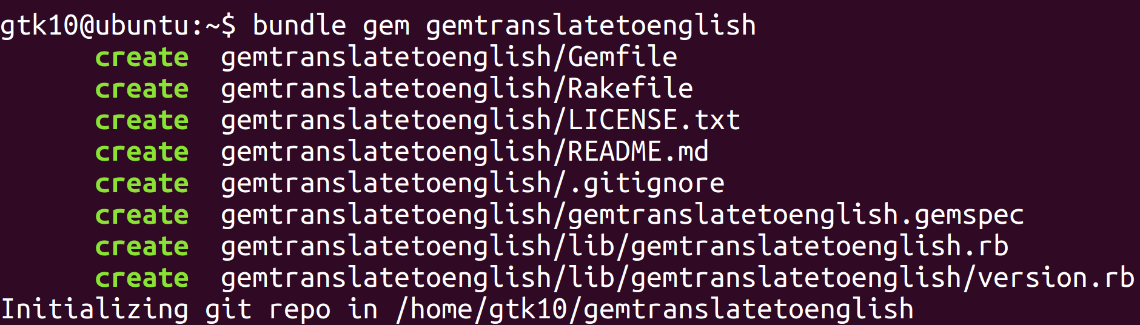
\includegraphics[scale=0.4]{images/execucao_que_cria_gema_gemtranslatetoenglish}
  \caption{Execução que cria gema gemtranslatetoenglish}
  \label{fig:execucao_que_cria_gema_gemtranslatetoenglish}
\end{figure}
\end{comment}

\subsubsection{Gemspec}
\label{subsubsection:gemspec}

Agora que possuimos a estrutura da gema, devemos fazer a edição do arquivo \emph{\textbf{gemspec}} 
para informar os dados básicos da gema e isso pode ser feito editando o arquivo ‘‘ 'nome da gema'.gemspec ''. 
No nosso exemplo fizemos a edição do arquivo ‘‘gemtranslatetoenglish.gemspec'' resultado no arquivo mostrado 
no código ‘‘Código \ref{lst:gemspec_gemtranslatetoenglish} - gemspec gemtranslatetoenglish''
%na imagem ‘‘Figura \ref{fig:gemspec_gemtranslatetoenglish} - gemspec gemtranslatetoenglish''
, onde cada linha será explicada com mais detalhes logo a seguir.

\lstinputlisting[ style=customBash, caption={gemspec gemtranslatetoenglish}, label={lst:gemspec_gemtranslatetoenglish}]
{codigos/gemtranslatetoenglish/gemtranslatetoenglish.gemspec}

\begin{comment}
\begin{figure}[ht]
  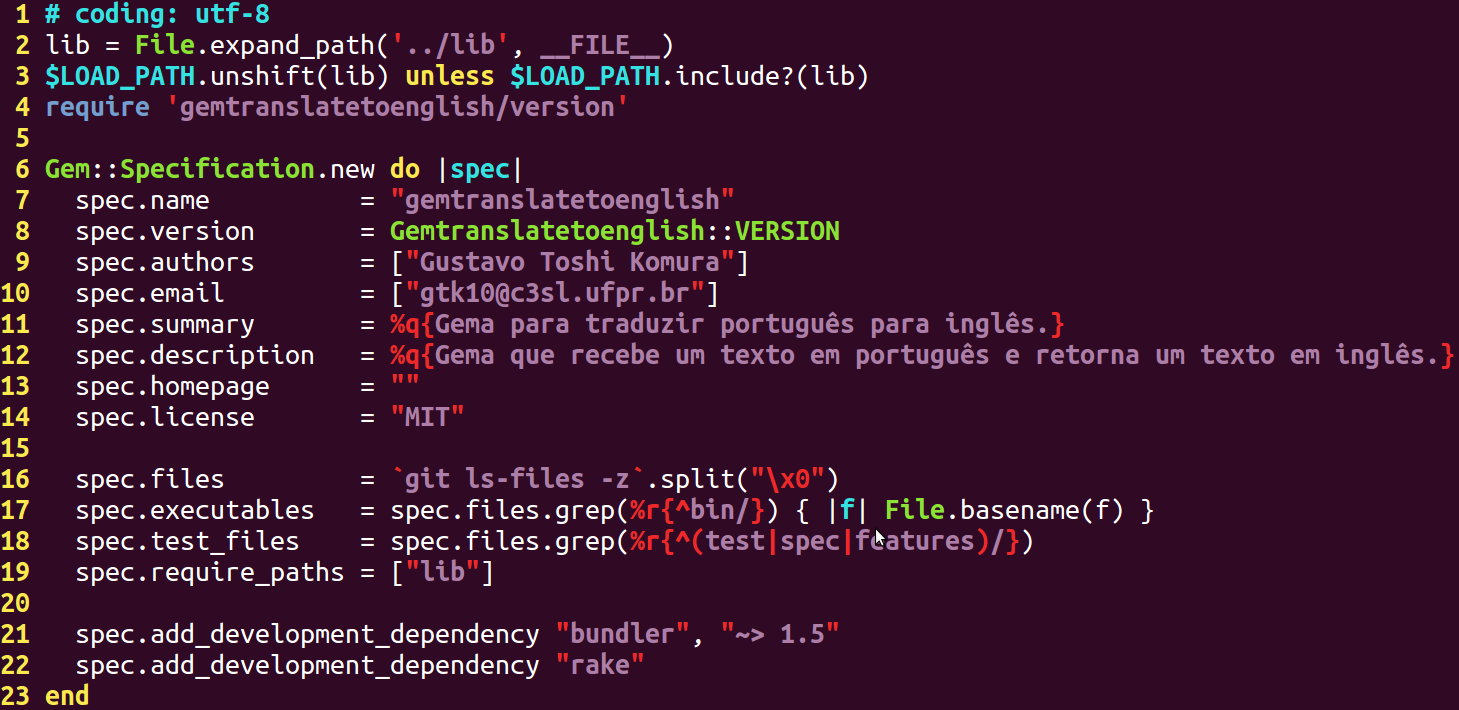
\includegraphics[scale=0.3]{images/gemspec_gemtranslatetoenglish}
  \caption{gemspec gemtranslatetoenglish}
  \label{fig:gemspec_gemtranslatetoenglish}
\end{figure}
\end{comment}

\begin{itemize}

 \item ‘‘\emph{\# coding: utf-8}'' na linha ‘‘1'' indica que o texto do arquivo está no formato \emph{UTF-8}.
 
 \item ‘‘\emph{lib = File.expand\_path('..\/lib', \_\_FILE\_\_)}'' na linha ‘‘2'' indica onde se encontra o 
 diretório \emph{\textbf{lib}} da gema.
 
 \item ‘‘\emph{\$LOAD\_PATH.unshift(lib) unless \$LOAD\_PATH.include?(lib)}'' na linha ‘‘3'' faz o 
 carregamento dos arquivos que estão no diretório \emph{\textbf{lib}} caso o diretório já esteja definido.
 
 \item ‘‘ \emph{require 'gemtranslatetoenglish/version'} '' na linha ‘‘4'' requisita o arquivo de versão da
 gema.
 
 \item ‘‘\emph{Gem::Specification.new do |spec|} ... end'' da linha ‘‘6'' a ‘‘23'' define a especifação da
 gema como \emph{spec}, ou seja, ao invés de escrever ‘‘\emph{Gem::Specification}'' a todo momento que for 
 definir uma especificação da gema se escreve somente ‘‘\emph{spec}''.
 
 \item ‘‘\emph{spec. }'' da linha ‘‘7'' a linha ‘‘14'' defini-se espcificações básicas da gema, como nome,
 versão, autor, e-mail do autor, breve descrição, descrição completa, página e tipo de licença.
 
 \item ‘‘\emph{spec.files = `git ls-files -z`.split("$\backslash$x0")}'' na linha ‘‘16'' indica os arquivos
 que devem ser incluídos na gema. Esses arquivos são incluídos dinâmicamente através do comando 
 ‘‘\emph{git ls-files -z}'' que traz como resultado todos os arquivos que estão naquele repositório 
 colocando entre as \emph{PATH}s deles o caracter ‘‘\emph{$\backslash$0}'' 
 (\emph{line termination on output}). Por consequência com a adição do comando \emph{Ruby} 
 ‘‘\emph{.split("$\backslash$x0")}'', que indica a divisão por ‘‘\emph{$\backslash$0}'', os arquivos 
 adicionados na gema são todos que estão no repositório. 
 
 Para se adicionar arquivos no repositório é necessário executar o comando ‘‘\emph{git add PATH}'', 
 onde \emph{PATH} é o caminho do arquivo que se deseja adicionar no repositório.
 
 \item ‘‘\emph{spec.executables = ...}'' e ‘‘\emph{spec.tes\_files = ...}'' nas linhas ‘‘17'' e ‘‘18'' 
 indicam os arquivos executáveis e os arquivos de teste respectivamente, e também indica que ambos devem
 ter permissão de execução, pois caso este arquivos não possuam essa permissão, eles não são incluídos 
 na gema.
 
 \item ‘‘\emph{spec.require\_paths = ["lib"]}'' requisita o diretório da \emph{\textbf{lib}} da gema.
 
 \item ‘‘\emph{spec.add\_development\_dependency = ...}'' nas linhas ‘‘21'', ‘‘22'' e ‘‘23'' requistam como 
 dependências as gemas ‘‘\emph{bundle}'' versão ‘‘1.5'', ‘‘\emph{rake}'' e ‘‘\emph{action\_controller}''
 respectivamente.
 
\end{itemize}

\subsubsection{Desenvolvimento de código de funcionalidade ou teste}
\label{subsubsection:desenvolvimento_de_codigo_de_funcionalidade_ou_teste}

Nesse momento podemos tomar 2 caminhos e isso depende da metodologia de projeto que adotadomos no inicio 
do desenvolvimento, ou seja, é nesse momento que podemos desenvolver o código das funcinalidades
ou implementar o código de testes. 

Na metodologia tradicional se faz a implementação do código de funcionalidades e depois se
desenvolve o código para testar essas funcionalidades. Por outro lado na metodologia voltada para 
testes, se implementa o código de testes para depois se desenvolver o código de funcionalidades.

Seguindo a metodologia tradicional, primeiramente iremos fazer o código das funcinalidades da gema.
Depois ao terminar de criar essas funcionalidades iremos elaborar os arquivos testes, mas nada o impede
de desenvolver os códigos de testes que serão apresentado na sub-sub-seção 
‘‘\ref{subsubsection:test_ou_spec_e_arquivo_rakefile} Test ou Spec e arquivo Rakefile'' antes de 
desenvolver os códigos de funcionalidade mostrados na sub-sub-seção ‘‘\ref{subsubsection:lib} Lib''.

\subsubsection{Lib}
\label{subsubsection:lib}

Nesta sub-seção vamos aprender a fazer o código de funcionalidade de uma gema, mas caso deseje fazer 
primeiro os códigos de casos de testes, pode-se consultar a sub-seção 
‘‘\ref{subsubsection:test_ou_spec_e_arquivo_rakefile} Test ou Spec e arquivo Rakefile'' e depois retornar
para esta sub-seção para dar continuidade ao desenvolvimento.

Caso esse código seja por meio de código \emph{Ruby} devemos fazer a edição e criação de arquivos no 
diretório \emph{\textbf{lib}}. Este diretório obrigatoriamente deve possuir um arquivo 
‘‘ 'nome da gema'.rb '' e um diretório também com o nome da gema. Dentro do diretório devemos criar um 
arquivo de versão. No nosso exemplo isso pode ser verificado consultando no código ‘‘Código 
\ref{lst:execucao_que_cria_gema_gemtranslatetoenglish} - Execução que cria gema gemtranslatetoenglish'' 
que após a execução do comando ‘‘\emph{bundle gem gemtranslatetoenglish}'' é feita a criação do arquivo 
‘‘\emph{lib/gemtranslatetoenglish.rb}'' na linha ‘‘8'', e o drietório ‘‘\emph{lib/gemtranslatetoenglish}'' 
com o arquivo ‘‘\emph{version}'' dentro dele na linha ‘‘9''.

O arquivo ‘‘\emph{version}'' somente define a versão que a gema está, onde no nosso exemplo da gema 
‘‘\emph{gemtranslatetoenglish}'' a primeira versão é a ‘‘\emph{0.0.1}''. 

Basicamente a descrição da versão de uma gema é uma string com números e pontos. Também é permitido 
colocar ao final a palavra chave ‘‘\emph{pre}'' caso seja um pré-lançamento de alguma versão, como 
por exemplo ‘‘\emph{1.0.0.pre}'' é um pré-lançamento da versão ‘‘\emph{1.0.0}''.

O \emph{Rubygems} recomenda seguir as seguintes politicas mencionadas logo abaixo que foram consultadas
em \emph{\href{http://guides.rubygems.org/patterns/\#semantic-versioning}{semantic-versioning}}
\footnote{semantic-version: \url{http://guides.rubygems.org/patterns/\#semantic-versioning}} e em
\emph{\href{http://guides.rubygems.org/specification-reference/\#version}{specification-reference-version}}
\footnote{specification-reference-version: \url{http://guides.rubygems.org/specification-reference/\#version}}.

\begin{itemize}
 \item PATH : “0.0.X” para pequenas alterações, como por exemplo correção de pequenos \emph{bugs}.
 \item MINOR: “0.X.0” para médias alterações, como por exemplo alteração/adição de funcionalidades.
 \item MAJOR: “X.0.0” para grandes alterações, como por exemplo remoção de alguma funcionalidade.
\end{itemize}

Antes de continuarmos a codificação das funcionalidades da gema precisamos entender algumas diferenças
básicas de conceitos do \emph{Ruby}, como por exemplo a diferença entre \emph{module} e \emph{class},

Os ‘‘\emph{modules}'' ou módulos se preferir, definem um conjunto de métodos e constantes. Podemos 
dizer que os métodos dos módulos são estáticos, pois não precisamos instanciar o módulo para usar os
seus métodos. Contudo podemos dizer que os módulos são parecidos com o conceito de interface do 
\emph{Java}. 

Por outro lado a ‘‘\emph{class}'' também é um conjunto de métodos e constantes, no 
entanto para usar os seus métodos e constantes é necessário instância-lá, ou seja, é necessário criar 
um objeto da ‘‘\emph{class}'' na memória para usar os seus respectivos métodos. 

Contudo por essas características podemos dizer que uma ‘‘\emph{class}'' é basicamente 
uma subclasse do ‘‘\emph{module}'', pois a ‘‘\emph{class}'' possui 4 métodos a mais, que no caso são 
os métodos ‘‘\emph{initialize()}'', ‘‘\emph{superclass()}'', ‘‘\emph{allocate()}'' e ‘‘\emph{to\_yank()}''.

Agora que temos alguns conceitos do \emph{Ruby} apresentados, podemos continuar com a implementação 
da nossa gema. 

No arquivo ‘‘ lib/'nome da gema'.rb '' temos a possibilidade de escerver todas as 
funcinalidades desejadas. No nosso exemplo o arquivo ‘‘lib/gemtranslatetoenglish.rb'' é mostrado no código 
‘‘Código \ref{lst:gemtranslatetoenglish.rb} - gemtranslatetoenglish.rb'', onde cada linha é explicado 
logo a seguir.

\lstinputlisting[ style=customRuby, caption={gemtranslatetoenglish.rb}, label={lst:gemtranslatetoenglish.rb}]
{codigos/gemtranslatetoenglish/lib/gemtranslatetoenglish.rb}

\begin{itemize}

 \item ‘‘\emph{require "gemtranslatetoenglish/version"} '' na linha ‘‘1'' é feita a requsição do arquivo de
 versão.
 
 \item ‘‘\emph{require "gemtranslatetoenglish/translatetoenglish.rb"} '' na linha ‘‘4'' é feita a requisição
 do arquivo ‘‘\emph{translatetoenglish.rb}'' contido no diretório ‘‘gemtranslatetoenglish''.
 
 \item ‘‘\emph{module Gemtranslatetoenglish ... end}'' na linha ‘‘6'' a ‘‘8'' define o módula da gema.
 
 \item ‘‘\emph{ActionController::Base.helper Gemtranslatetoenglish::Helpers::Translatetoenglish}'' na linha 
 ‘‘10'' define uma extensão da classe ‘‘ActionController::Base.helper'', onde a classe a ser acrescentada é
 a classe ‘‘\emph{Gemtranslatetoenglish::Helpers::Translatetoenglish}''. Esta extensão foi adicionada
 para que no momento de uso das funcionalidades da gema na \emph{view} não fosse necessário fazer a chamada 
 de tradução  escrevendo toda \emph{PATH}. Por exemplo para chamar a função de tradução, ao invés
 de chamar ‘‘\emph{gemtranslatetoenglish.Translatetoenglish.translate(‘Oi’)}'', se faz a chamada 
 ‘‘\emph{translate(‘Oi’)}'' na \emph{view}.
 
\end{itemize}

Podemos perceber que o comando ‘‘\emph{require}'' é utilizado para fazer a chamada de código de outros 
arquivos e isso serve para fazer a modularização da gema que no caso é uma boa prática de programação.

Podemos supor que desenvolvemos uma gema e depois de um certo tempo precisamos fazer a manutenção do 
seu código. Neste caso se não modularizamos a gema, a correção de \emph{bugs} ou mesmo a adição de 
novas funcionalidades torna-se uma tarefa muito complexa, pois não existe nenhuma organização 
estrutural na gema preparada para facilitar esse tipo de operação. 

Observando novamente o código ‘‘Código \ref{lst:gemtranslatetoenglish.rb} - gemtranslatetoenglish.rb'' 
podemos perceber que na linha ‘‘4'' foi feito o \emph{require} do arquivo 
‘‘\emph{gemtranslatetoenglish/translatetoenglish.rb}'' que será mostrado no código ‘‘Código 
\ref{lst:translatetoenglish.rb} - translatetoenglish.rb'' e explicado logo a seguir.

\lstinputlisting[ style=customRuby, caption={translatetoenglish.rb}, label={lst:translatetoenglish.rb}]
{codigos/gemtranslatetoenglish/lib/gemtranslatetoenglish/translatetoenglish.rb}

\begin{itemize}

  \item ‘‘\emph{module ... end} nas linhas ‘‘1'', ‘‘2'' e ‘‘3'' até as linhas ‘‘44'', ‘‘45'' e ‘‘46'' 
  define a árvore de módulos ‘‘\emph{Gemtranslatetoenglish}'' na raiz, ‘‘\emph{Helpers}'' no segundo 
  nível e depois ‘‘\emph{Translatetoenglish}'' no terceiro nível.
  \item ‘‘\emph{def translate( phrase) ... end}'' da linha ‘‘5'' até a linha ‘‘42'' define a função de 
  tradução da gema, onde foi definido somente duas traduções, ‘‘\emph{OI}'' para ‘‘\emph{HELLO}'' 
  e ‘‘MUNDO'' para ‘‘\emph{WORLD}''.
  
  A árvore definida no código ‘‘Código \ref{lst:translatetoenglish.rb} - translatetoenglish.rb'' foi 
  necessário por causa do código inserido na linha ‘‘10'' 
  ‘‘\emph{ActionController::Base.helper Gemtranslatetoenglish::Helpers::Translatetoenglish}''
  no código ‘‘Código \ref{lst:gemtranslatetoenglish.rb} - gemtranslatetoenglish.rb'' que serve para 
  evitar a necesseidade de escrever a \emph{PATH} completa na \emph{view} para chamar uma função 
  da gema na \emph{view}.
  
\end{itemize}

\subsubsection{Test ou Spec e arquivo Rakefile}
\label{subsubsection:test_ou_spec_e_arquivo_rakefile}

Lembrando que podemos fazer o desenvolvimento de código de funcinalidades ou o código de testes, e isso é
dependente da metodologia adotada no inicio do projeto, caso queira fazer o código de funcionalidade antes
do desenvolvimento dos casos de teste se pode consutar a sub-seção ‘‘\ref{subsubsection:lib} Lib''.

Para se fazer os testes, deve-se criar os arquivos de testes dentro do diretório ‘‘\emph{test}'' ou se 
preferir ‘‘\emph{spec}''. Não existe um padrão especificado, mais recomenda-se criar um arquivo de 
teste com o nome ‘‘\emph{test/test\_‘definição do teste'.rb}''. No nosso exemplo criamos o arquivo 
‘‘\emph{test/test\_check\_translate.rb}'' que podemo ver no código ‘‘\ref{lst:test_check_translate.rb} - 
Testa translate gemtranslatetoenglish'' explicado logo a seguir.

\lstinputlisting[ style=customRuby, caption={Testa translate gemtranslatetoenglish}, label={lst:test_check_translate.rb}]
{codigos/gemtranslatetoenglish/test/test_check_translate.rb}

\begin{itemize}

 \item Nas linhas ‘‘1'', ‘‘2'' e ‘‘3'' nos códigos ‘‘ \emph{require ‘...'} '' requisitamos respectivamente o 
 ‘‘\emph{autorun}'' da gema ‘‘\emph{minitest}'' que utilizaremos para realizar os testes, 
 ‘‘\emph{action\_controller}'' que utilizamos para evitar a obrigação de digitar a ‘‘\emph{PATH}'' completa 
 na \emph{view}, e ‘‘\emph{gemtranslatetoenglish}'' que é a nossa gema de exemplo.
 
 \item Na linha ‘‘5'' fomos obrigados a fazer o ‘‘\emph{include}'' do módulo 
 ‘‘\emph{Gemtranslatetoenglish::Helpers::Translatetoenglish}'' para que todas as funções do módulo fossem 
 disponiblizadas para uso e no nosso caso era o método ‘‘\emph{translate()}''.
 
 \item Da linha ‘‘7'' a linha ‘‘16'' é definido a classe de teste \emph{TranslateTest} que herda as 
 características de ‘‘\emph{MiniTest::Unit::TestCase}''.
 
 \item Da linha ‘‘8'' a linha ‘‘11'' é definido o teste por palavra, onde é verificado através do 
 ‘‘\emph{assert\_equal}'' se a ‘‘\emph{string}'' esperada no primeiro parâmetro é retornadda pela chamada 
 da função ‘‘\emph{Gemtranslatetoenglish::Helpers::Translatetoenglish.translate()}'' no segundo parâmetro.
  
 \item Da linha ‘‘12'' a linha ‘‘15'' é definido o teste por texto, onde é verificado através do 
 ‘‘\emph{assert\_equal}'' se a ‘‘\emph{string}'' esperada no primeiro parâmetro é retornadda pela chamada 
 da função ‘‘\emph{Gemtranslatetoenglish::Helpers::Translatetoenglish.translate()}'' no segundo parâmetro.
 
\end{itemize}

Agora que temos o nosso arquivo de teste, precisamos criar o arquivo ‘‘\emph{Rakefile}'' e executar o 
comando ‘‘\emph{rake}'' para realizarmos os testes.

No nosso exemplo da gema ‘‘\emph{gemtranslatetoenglish}'' desenvolvemos o seguinte arquivo 
‘‘\emph{Rakefile}'' que pode ser visualizado no código ‘‘Código \ref{lst:rakefile} - 
Rakefile gemtranslatetoenglish'' sendo explicado os detalhes logo a seguir.

\lstinputlisting[ style=customRuby, caption={Rakefile gemtranslatetoenglish}, label={lst:rakefile}]
{codigos/gemtranslatetoenglish/Rakefile}

\begin{itemize}

\item Nas linhas ‘‘1'' e ‘‘2'' nos códigos ‘‘ \emph{require ‘...'} '' requisitamos respectivamente o 
 ‘‘\emph{gem\_tasks}'' do ‘‘\emph{bundler}'' e ‘‘\emph{testtask}'' do ‘‘\emph{rake}'', ambos necessários para
 a execução dos testes.
 
 \item Da linha ‘‘4'' a ‘‘6'' é feito a criação de uma nova ‘‘\emph{task}'' de teste para cada arquivo 
 que esteja no diretório ‘‘\emph{test}''.
 
 \item A linha ‘‘5'' com o código ‘‘ \emph{t.libs << ‘test'} '' inidica que os arquivos de testes estão no 
 diretório ‘‘\emph{test}''.

 \item Por fim na linha ‘‘9'' com o código ‘‘\emph{task :default => :test}'' se requisita a execução 
 dos testes.
 
\end{itemize}

\subsubsection{Execução de testes}
\label{subsubsection:execução_de_testes}

Antes de realizarmos os testes, precisamos criar a gema com comando ‘‘\emph{gem build 'nome da gema'.gemspec}'' 
e fazer a instalação com o comando ‘‘\emph{sudo gem install 'nome da gema'-'versão da gema'.gem}''. No nosso 
caso é fazer a crição e a instalação da gema ‘‘\emph{gemtranslatetoenglish}'', que pode ser feito da mesma 
forma como apresentado no código ‘‘Código \ref{lst:execucao_que_cria_e_instala_gemtranslatetoenglish} - Execução 
gem install gemtranslatetoenglish''.

\lstinputlisting[ style=customBash, caption={Execução que Cria e Instala gemtranslatetoenglish}, label={lst:execucao_que_cria_e_instala_gemtranslatetoenglish}]
{codigos/execucao_que_cria_e_instala_gemtranslatetoenglish.sh }

Agora após ter implementado o código das funcionalidades, o arquivo de teste 
‘‘\emph{test/test\_check\_translate.rb}'', o arquivo \emph{Rakefile}, e ter feito a criação e a instalação 
da gema de exemplo, podemos realizar os testes com a execução do comando ‘‘\emph{rake}'' no terminal. 

Com a execução dos testes obtemos como resultado o código ‘‘Código 
\ref{lst:execucao_rake_gema_gemtranslatetoenglish} - Execução rake gema gemtranslatetoenglish'' explicado 
logo a seguir.

\lstinputlisting[ style=customBash, caption={Execução rake gema gemtranslatetoenglish}, label={lst:execucao_rake_gema_gemtranslatetoenglish}]
{codigos/execucao_rake_gema_gemtranslatetoenglish.sh }

\begin{itemize}

 \item Na linha ‘‘1'' é feito a execução do comando ‘‘\emph{rake}'' para se realizar os testes.
 
 \item Na linha ‘‘9'' é mostrado que foram feitos 2 testes, no caso os 2 que definimos no código 
 ‘‘\ref{lst:test_check_translate.rb} - Testa translate gemtranslatetoenglish'' nas linhas 
 ‘‘8'' a ‘‘11'' no teste ‘‘\emph{test\_world\_translation}'' e nas linhas ‘‘12'' a ‘‘15'' no teste 
 ‘‘\emph{test\_text\_translation}''. Também é apresentado na linha ‘‘9'' que foram feitos 4 
 ‘‘\emph{assertions}'', no caso dois para cada caso de teste feitos por meio do ‘‘\emph{assert\_equal}''.
 E além disso é apresentado que não ocorreram  \emph{failures}''), ‘‘\emph{errors}'' e ‘‘\emph{skips}''.
 
\end{itemize}

Deste modo ao se realizar estes testes garantimos que pelo menos a função ‘‘\emph{translate()}'' da gema
‘‘\emph{gemtranslatetoenglish}'' esta funcionando como o esperado.

Contudo no momento do desenvolvimento do código de testes, o aconselhável é para cada função adicionada 
na gema, fazer testes com todas as possíveis entradas, verificando se o resultado para cada entrada 
está correto.

\subsubsection{IRB}
\label{subsubsection:irb}

O \emph{\href{http://www.ruby-doc.org/stdlib-2.0/libdoc/irb/rdoc/IRB.html}{IRB}} 
\footnote{IRB: \url{http://www.ruby-doc.org/stdlib-2.0/libdoc/irb/rdoc/IRB.html}}
(\emph{Interactive Ruby Shell}) é uma ferramenta do \emph{Ruby} que serve para executar expressões
interativamente, fazendo a leitura da entrada padrão [\citeonline{irb_doc}].

Caso se deseje fazer os testes de uma gema manualmente sem a necessidade de inclui-lá em um projeto, podemos
fazer o uso do ‘‘\emph{IRB}'', chamando o comando ‘‘\emph{irb}''.
% o seguinte comando mostrado no código ‘‘Código \ref{lst:executa_irb} - Executa IRB'' no terminal para iniciá-lo.

\begin{comment}
\lstinputlisting[ style=customBash, caption={Executa IRB}, label={lst:executa_irb}]
{codigos/executa_irb.sh}
\end{comment}

Um exemplo de uso do \emph{IRB} pode ser visto 
% na imagem ‘‘Figure \ref{fig:exemplo_de_uso_do_irb} - Exemplo de Uso do IRB'' 
no código ‘‘Código \ref{lst:exemplo_de_uso_do_irb} - Exemplo de Uso do IRB''
abaixo, explicado em mais detalhes na listagem abaixo. 

\begin{comment}
\begin{figure}[ht]
  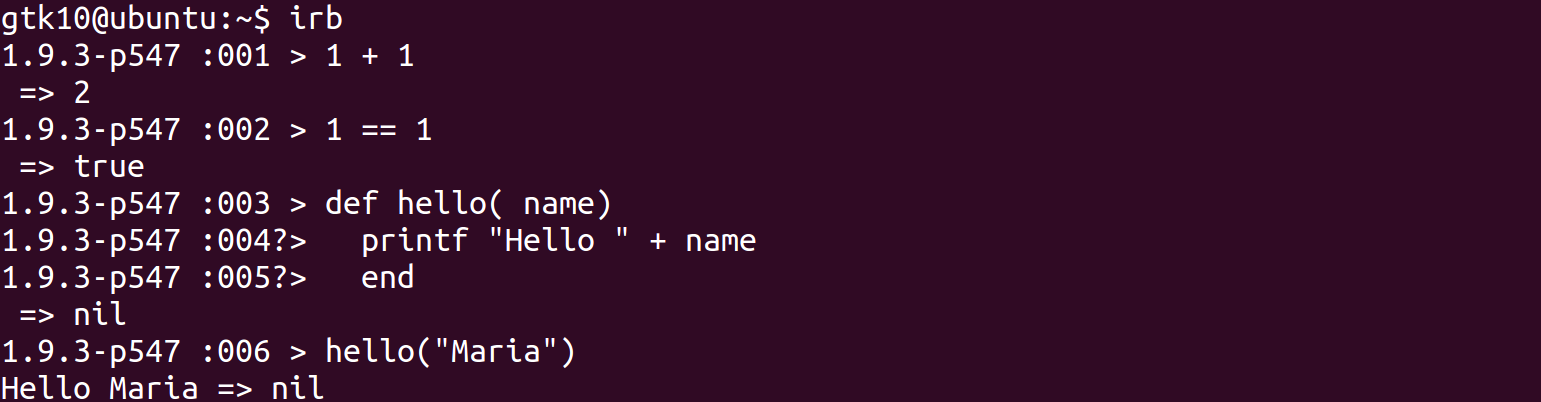
\includegraphics[scale=0.3]{images/exemplo_de_uso_do_irb}
  \caption{Exemplo de Uso do IRB}
  \label{fig:exemplo_de_uso_do_irb}
\end{figure}
\end{comment}

\lstinputlisting[ style=customBash, caption={Exemplo de uso do IRB}, label={lst:exemplo_de_uso_do_irb}]
{codigos/exemplo_de_uso_do_irb.sh}

\begin{itemize}

\begin{comment}
 \item Primeiramente é feita a chamada da ferramenta \emph{IRB} com o comando ‘‘\emph{irb}'' no terminal.
 
 \item Depois é requisitado a soma entre ‘‘\emph{1 + 1}'' resultando em ‘‘\emph{2}''.
 
 \item Em seguida é perguntado se ‘‘\emph{1 == 1}'' resultando em ‘‘\emph{true}''.

 \item E no fim é criado uma função chamada de ‘‘\emph{hello}'' com o parâmetro ‘‘\emph{name}'' e ao se 
 chamar essa função é devolvido na tela ‘‘\emph{Hello +}'' o parâmetro passado para a função. O resultado
 pode ser visto quando se requisita ‘‘\emph{hello(‘‘Maria'')}'' e se obtem como resultado 
 ‘‘\emph{Hello Maria}''.
\end{comment}
 
  \item Primeiramente na linha ‘‘1'' é feita a chamada da ferramenta \emph{IRB} com o comando ‘‘\emph{irb}'' 
  no terminal.
 
 \item Depois na linha ‘‘2'' é requisitado a soma entre ‘‘\emph{1 + 1}'' resultando em ‘‘\emph{2}'' na linha 
 ‘‘3''.
 
 \item Em seguida na linha ‘‘4'' é verificado se ‘‘\emph{1 == 1}'' resultando em ‘‘\emph{true}'' na linha 
 ‘‘5''.

 \item E no fim entre as linhas ‘‘6'' e ‘‘8'' é criado uma função chamada de ‘‘\emph{hello}'' com o 
 parâmetro ‘‘\emph{name}'' e ao se chamar essa função é devolvido na tela ‘‘\emph{Hello}'' mais o 
 parâmetro passado para a função. O resultado pode ser visto quando se requisita 
 ‘‘\emph{hello(‘‘Maria'')}'' na linha ‘‘10'', obtendo como resultado ‘‘\emph{Hello Maria}'' na linha ‘‘11''.
 
\end{itemize}

No nosso exemplo da gema ‘‘\emph{gemtranslatetoenglish}'' fizemos alguns testes simples mostrados
na código ‘‘Código \ref{lst:teste_irb_da_gema_gemtranslatetoenglish} - Teste IRB da gema 
gemtranslatetoenglish'' explicado com mais detalhes nos itens abaixo.

\begin{comment}
\begin{figure}[ht]
  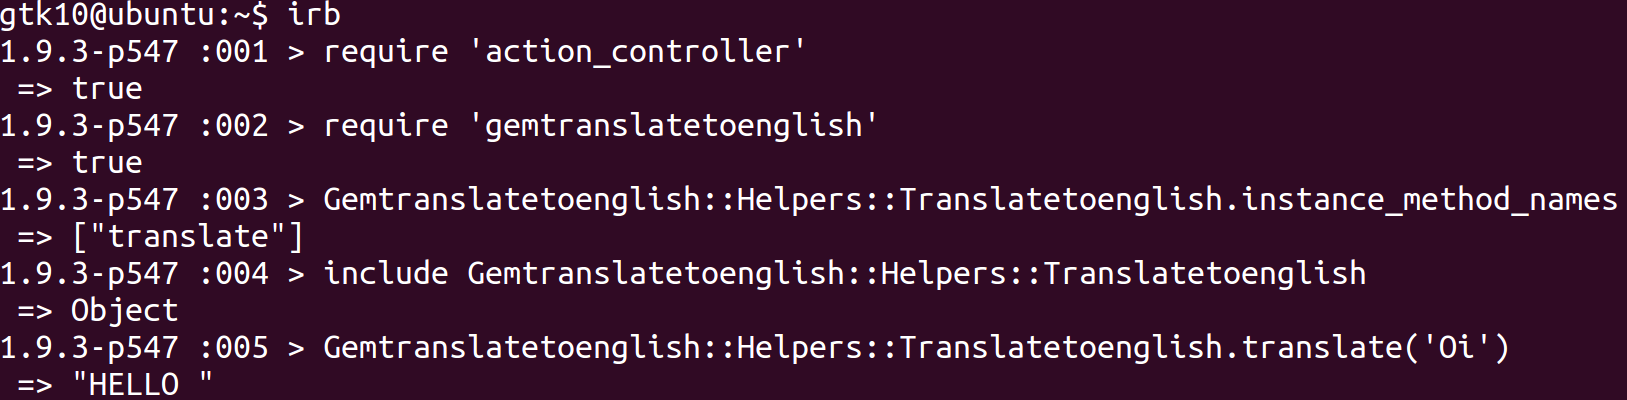
\includegraphics[scale=0.28]{images/teste_irb_da_gema_gemtranslatetoenglish.png}
  \caption{Teste IRB da gema gemtranslatetoenglish}
  \label{fig:teste_irb_da_gema_gemtranslatetoenglish}
\end{figure}
\end{comment}

\lstinputlisting[ style=customBash, caption={Teste IRB da gema gemtranslatetoenglish}, label={lst:teste_irb_da_gema_gemtranslatetoenglish}]
{codigos/teste_irb_da_gema_gemtranslatetoenglish.sh}

\begin{itemize}

 \item Primeiramente na linha ‘‘1'' é feita a chamada da ferramenta \emph{IRB} com o comando ‘‘\emph{irb}'' 
  no terminal.
  
  \item Na linha ‘‘2'' é executado o comando ‘‘ \emph{require 'action\_controller'} '' para buscar a gema 
  ‘‘\emph{ActionController}'' necessária no uso da nossa gema de exemplo quando evitamos digitar a 
  \emph{PATH} completa na ‘‘\emph{view}''.

  \item Na linha ‘‘4'' é executado o comando ‘‘ \emph{require 'gemtranslatetoenglish'} '' para buscar a 
  nossa gema de exemplo.
  
  \item Na linha ‘‘6'' é executado o comando 
  ‘‘ \emph{instance\_method\_names}'' para verificar se o nosso método \emph{translate()} existe.
  
  \item Na linha ‘‘8'' é executado o comando ‘‘\emph{include}'' para incluir as funções do módulo 
  ‘‘\emph{Translatetoenglish}''.
  
  \item Na linha ‘‘10'' é executado o comando 
  ‘‘\emph{translate('Oi')}'' para verificar se a função funciona como o esperado.
  
  \item E no fim na linha ‘‘11'' podemos verificar que a função \emph{translate()} funcionou corretamente,
  pois obtemos como resultado a palavra ‘‘\emph{HELLO }''.
  
 \end{itemize}

\subsubsection{Exemplo de uso de gemtranslatetoenglish}
\label{subsubsection:exemplo_de_uso_de_gemtranslatetoenglish}

Até o momento falamos muito da utilização do \emph{action\_controller} para simplificar o uso da função 
\emph{translate()} na \emph{view}, e agora vamos apresentar essa facilidade através de um exemplo, 
fazendo o uso da gema ‘‘\emph{gemtranslatetoenglish}'' em um projeto.

O primeiro passo é criar um projeto no \emph{framework rails} e isso pode ser feito executando 
o seguinte comando apresentado no código ‘‘Código 
\ref{lst:executa_rails_new_para_gemtranslatetoenglish} - Executa rails new para gemtranslatetoenglish''
explicado logo a seguir.

\lstinputlisting[ style=customBash, caption={Executa rails new para gemtranslatetoenglish}, label={lst:executa_rails_new_para_gemtranslatetoenglish}]
{codigos/executa_rails_new_para_gemtranslatetoenglish_simplificado.sh} 

\begin{itemize}

 \item O comando ‘‘\emph{rails new}'' implica na criação de um projeto básico do \emph{Ruby On Rails}.
 
 \item O nome ‘‘\emph{projeto\_teste\_gemtranslatetoenglish}'' é o nome do proejto a ser criado.
 
  \item Os códigos a partir da linha ‘‘2'' não representam execuções. No caso estes códigos somente 
 mostram os passos realizados por causa da execução do comando na primeira linha.
 
 \item A execução deste comando implica na criação de alguns diretórios e arquivos e por simplificação 
 somente explicaremos aqueles que vamos utilizar neste exemplo:
  
  \subitem - ‘‘\emph{Gemfile}'' arquivo que contém as \emph{gemas} que são utilizadas no projeto.
 
  \subitem - ‘‘\emph{config/routes.rb}'' arquivos que possui as rotas utilizadas no projeto.
 
\end{itemize}

Agora que criamos o projeto, precisamos fazer a criação de pelo menos um \emph{controller} e uma \emph{view}.
O \emph{controller} serve para receber uma requisição e determinar a partir dos parâmetros desta 
requisição, a \emph{view} e os dados que devem ser apresentados. A \emph{view} serve para 
determinar um formato e mostrar os dados no \emph{browser}.

Para o nosso exemplo criamos o \emph{controller} ‘‘traducao'' e a \emph{view} ‘‘index'' com a execução do 
comando que pode ser visto no código ‘‘Código \ref{lst:executa_rails_generate_para_gemtranslatetoenglish} - 
Executa rails generate para gemtranslatetoenglish'' explicado logo a seguir.

\lstinputlisting[ style=customBash, caption={Executa rails generate para gemtranslatetoenglish}, label={lst:executa_rails_generate_para_gemtranslatetoenglish}]
{codigos/executa_rails_generate_para_gemtranslatetoenglish.sh} 

\begin{itemize}

 \item Na linha ‘‘1'' é feito a execução do comando ‘‘\emph{rails generate controller traducao index}'' no 
 terminal para gerar o \emph{controller} ‘‘\emph{traducao}'', e a \emph{view} ‘‘\emph{index}'' para 
 ‘‘\emph{traducao}''.

 \item Os códigos a partir da linha ‘‘2'' não representam execuções. No caso estes códigos somente 
 mostram os passos realizados por causa da execução do comando na primeira linha.
 
 \item Na linha ‘‘2'' foi criado o \emph{controller} com o nome ‘‘\emph{traducao\_controller.rb}''
 
 \item Na linha ‘‘3'' foi adicionado no arquivo ‘‘\emph{config/routes.rb} o método \emph{get} para a 
 \emph{view} ‘‘\emph{traducao/index}''.
 
 \item Na linha ‘‘6'' foi criado a \emph{view} ‘‘\emph{traducao/index.html.erb}''.
 
 \item A partir da linha ‘‘7'' são criados os arquivos de teste funcional, os \emph{helpers}, e os 
 \emph{assets} que possuem códigos \emph{coffeescript} que depois vão se tornar \emph{javascript} e 
 \emph{scss} que depois vão se tornar \emph{css}.
 
\end{itemize}


Agora para fazer o uso da nossa gema de exemplo em um projeto feito no \emph{Ruby On Rails}, basta fazer a 
inclusão da gema no final do arquivo \emph{Gemfile} da mesma forma como mostrado no código ‘‘Código 
\ref{lst:adiciona_gemtranslatetoenglish_no_gemfile} - Adiciona gemtranslatetoenglish no Gemfile''
 
 \lstinputlisting[ style=customRuby, caption={Adiciona gemtranslatetoenglish no Gemfile}, label={lst:adiciona_gemtranslatetoenglish_no_gemfile}]
{codigos/adiciona_gemtranslatetoenglish_no_gemfile}
 
Agora que a gema ‘‘\emph{gemtranslatetoenglish}'' já esta incluída no nosso projeto, podemos fazer o uso 
dela em uma \emph{view} da seguinte maneira apresentada no código ‘‘Código 
\ref{lst:exemplo_do_translate_na_view} - Exemplo do translate() na view'' explicado logo a seguir.

\lstinputlisting[ style=customRubyHTML, caption={Exemplo do translate() na view}, label={lst:exemplo_do_translate_na_view}]
{codigos/projeto_teste_gemtranslatetoenglish/app/views/traducao/index.html.erb} 
 
 \begin{itemize}
 
  \item As linhas ‘‘1'' e ‘‘2'' já existiam, pois foram criadas automaticamente após a execução do comando 
  ‘‘\emph{rails generate controller traducao index}'' que mostramos no código ‘‘Código 
  \ref{lst:executa_rails_generate_para_gemtranslatetoenglish} - Executa rails generate para 
  gemtranslatetoenglish''.
  
  \item Na linha ‘‘4'' inserimos uma \emph{tag <p>} indicando para o \emph{browser} que vamos inserir um 
  texto. Depois inserimos a \emph{tag <\%= ... \%>} que indica que entre essas \emph{tags} será inserido um 
  código \emph{Ruby}. E dentro destas \emph{tags} chamamos o nosso método \emph{translate()} da gema 
  ‘‘\emph{gemtranslatetoenglish}'' com o parâmetro ‘‘Oi Mundo''.
  
 \end{itemize}

Agora que temos a nossa função ‘‘\emph{translate()}'' dentro da \emph{view} ‘‘\emph{traducao/index}'', podemos 
verificar se a tradução funciona corretamente. Para isso devemos dentro do diretório do nosso projeto,
iniciar o servidor no terminal através do comando ‘‘\emph{rails server -p2342}'', onde o parâmetro ‘‘-p2342'' 
indica que o servidor vai usar a porta ‘‘2342''. 

Depois com o servidor funcionando, podemos verificar na imagem ‘‘Figure \ref{fig:resultado_de_translate_na_view} - 
Resultado de Translate na View'' que ao se acessar o endereço ‘‘localhost:2342/traducao/index'' no 
\emph{browser}, a nossa função de tradução funciona corretamente, pois na página é apresentado o 
texto ‘‘HELLO WORLD''.
 
 \begin{figure}[ht]
  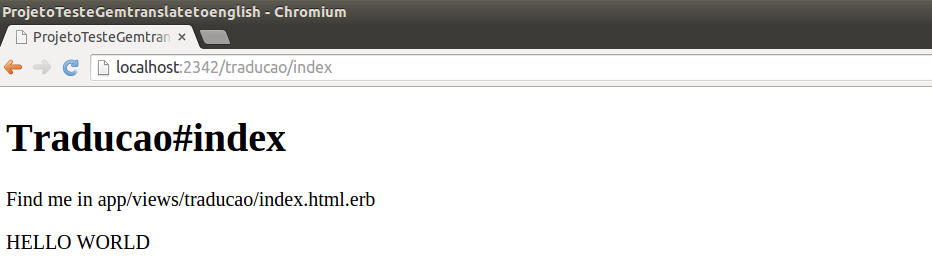
\includegraphics[scale=0.49]{images/resultado_de_translate_na_view.png}
  \caption{Resultado de Translate na View}
  \label{fig:resultado_de_translate_na_view}
\end{figure}
 
\section{Adaptando uma gema}
\label{section:adaptando_uma_gema}

Agora que sabemos como criar uma gema visto na seção ‘‘\ref{section:criando_uma_gema} - Criando uma gema'', 
podemos partir para a ideia de fazer modificações em uma gema que já existe, ou seja, fazer a adaptação de 
uma gema adicionando novas funcionalidade que geralmente utilizamos. 

Suponha o cenário aonde utilizamos com frequência uma certa gema, no entanto apesar dela comportar várias 
funcionalidades, ela não possui tudo que desejamos. Neste caso basta fazer a adaptação desta gema, não 
sendo necessário criar uma nova gema do zero, isso desde que a funcionalidade que precisamos 
esteja no mesmo contexto abordado pela gema. 

Por exemplo se estamos utilizando uma gema matemática e ela não possuir uma função para calcular a 
raiz de um número, podemos fazer uma modificação nesta gema para que ela possa calcular a raiz. 
No entanto não faz nenhum sentido incluuir uma funcionalidade de criar mapas do \emph{Google}, pois 
não está no mesmo contexto da gema.

Para facilitar o entendimento utilizaremos para a explicação a gema 
\emph{\href{https://github.com/toshikomura/Google-Maps-for-Rails}{Google-Maps-for-Rails}} 
\footnote{Google-Maps-for-Rails : \url{https://github.com/toshikomura/Google-Maps-for-Rails}} que é um 
\emph{branch} da gema 
\emph{\href{https://github.com/apneadiving/Google-Maps-for-Rails}{Google-Maps-for-Rails}} 
\footnote{Google-Maps-for-Rails : \url{https://github.com/apneadiving/Google-Maps-for-Rails}} criada por 
\emph{\href{https://github.com/apneadiving}{Benjamin Roth}} 
\footnote{Bejamin Roth: \url{https://github.com/apneadiving}} e 
\emph{\href{https://github.com/MrRuru}{David Ruyer}} \footnote{David Ruyer: \url{https://github.com/MrRuru}}.

Essa gema criada por \emph{Bejamin Roth} e \emph{David Ruyer} tem como objetivo criar mapas de forma 
simplificada, proporcionando a inclusão de sobreposições oferecidas pelo \emph{Google} como por exemplo 
marcadores e circulos. Ela também possui um código bem flexível que permite a aceitação de outros 
provedores de mapas [\citeonline{google_maps_for_rails}].

\subsection{API do Google Maps} 
\label{subsection:api_do_google_maps} 
 
Para fazer a adaptação da gema foi necessário fazer um estudo sobre como utilizar a \emph{API} do 
\emph{Google} e para isso foi utilizado como base o livro \emph{Beginning Google Maps API 3} 
[\citeonline{beginning_google_maps_api3}] e a 
\emph{\href{https://developers.google.com/maps/}{Google Maps API V3}} 
\footnote{Google Maps API V3: \url{https://developers.google.com/maps/}}, onde ambos se complementam 
ensinando os passos básicos para criar e manipular mapas do \emph{Google}. 

O \emph{Google Maps} e sua respectiva \emph{API} foram criadas por dois irmãos \emph{Lars} e 
\emph{Jens Rasmussen}, cofundadores da ‘‘\emph{Where 2 Technologies}'', compania dedicada a criação de mapas
que foi comprada pelo \emph{Google} em 2004 [\citeonline{beginning_google_maps_api3}].

Até o inicio do ano 2005 a rederização de mapas pela rede possuía um alto custo, necessitando de 
servidores altamente equipados para suportar a carga de trabalho. Mas em Fevereiro de 2005 através 
de um \emph{post} em seu \emph{blog}, o \emph{Google} anunciou uma nova solução de rederização, 
possiblitando ao usuário interagir com um mapa em uma página \emph{web}
[\citeonline{beginning_google_maps_api3}].

Depois de fazer o lançamento da nova forma para criar mapas, o \emph{Google} percebeu que 
muitos desenvolvedores gostariam de incorporar essa nova solução em seus projetos, e por esse 
movtio em Junho de 2005 anunciou a primeira versão pública da \emph{API} do \emph{Google Maps}
[\citeonline{beginning_google_maps_api3}].

O \emph{Google Maps} funciona de uma forma bem simples fazendo a criação e a manipulação do mapa
por meio de \emph{HTML}, \emph{CSS} e \emph{Javascript}. Basicamente o usuário por meio do \emph{browser}
requisita algum local do mapa informando a coordenada e o zoon desejado. Desta forma o servidor retorna a 
imagem do mapa que representa a posição requisitada [\citeonline{beginning_google_maps_api3}]. 

\subsection{Engenharia Reversa}
\label{subsection:engenharia_reversa}

Para conseguirmos entender o funcionamento de uma gema, precisamos obrigatoriamente fazer uma tradução
do código fonte para diagramas, pois não conseguiremos fazer nenhuma modificação consistente
se não tivermos uma visão geral de seu funcionamento, e esse procedimento de tradução se chama 
\emph{engenharia reversa}.

\emph{Engenharia reversa} é um processo de análise para a extração de informações de algo que já 
existe em um modelo de abstração de alto nível. Essas informações podem estar no formato de código 
fonte ou mesmo em um executável. O processo de análise para a extração de dados deve ser feita de forma
minunciosa, pois pode ocorrer uma grande perda de recursos, caso alguma funcionalidade seja entendida de
forma incorreta. E o modelo de abstração de alto nível pode ser por exemplo um diagrama de caso de uso ou
um diagrama de sequência.

Aplicando a \emph{engenharia reversa} na gema \emph{Google-Maps-For-Rails} conseguimos obter como resultado
os diagrama de classe na imagem ‘‘Figure \ref{fig:diagrama_de_classes_google_maps_for_rails} - Diagrama de 
Classes Google-Maps-For-Rails'', o diagrama de atributos na imagem ‘‘Figure - 
\ref{fig:diagrama_de_atributos_google_maps_for_rails} - Diagrama de Atributos Google-Maps-For-Rails'' e o 
diagrama de herança na imagem ‘‘Figure - \ref{fig:diagrama_de_heranca_google_maps_for_rails} - Diagrama de 
Herança Google-Maps-For-Rails'' que serão explicados em mais detalhes logo a seguir.

Nenhum dos 3 diagramas segue os seus respectivos padrões e isso deve ao fato de que não existia espaço 
suficiente na imagem para representar o sistema da gema por completo. Por esse motivo optamos por definir 
novos diagramas que possuem características sinilares aos seus padrões, mas com algumas características
adicionais.

Para as imagens de diagrama de classes ‘‘Figure \ref{fig:diagrama_de_classes_google_maps_for_rails} - 
Diagrama de Classes Google-Maps-For-Rails'' e o diagrama de atributos na imagem ‘‘Figure - 
\ref{fig:diagrama_de_atributos_google_maps_for_rails} - Diagrama de Atributos Google-Maps-For-Rails''
as seguintes explicações são válidas:

\begin{itemize}

 \item Cada retângulo representa uma classe da gema.
 
 \item O nome ácima dos traços ‘‘-----'' representa o nome da classe.
 
 \item O símbolo ‘‘*'' do lado esquerdo do nome da classe representa que ela é \emph{superclasse} e o 
 símbolo ‘‘*'' do lado direito do nome da classe representa que ela é uma \emph{subclasse}, por exemplo
 ‘‘\emph{* Objects.BaseBuilder}'' é \emph{superclasse} de ‘‘\emph{Google.Builders.Map *}'', neste caso 
 ‘‘\emph{Google.Builders.Map *}'' é \emph{subclasse} de ‘‘\emph{* Objects.BaseBuilder}''. O mesmo 
 critério é válido para o símbolo ‘‘\$''.
 
 \item O símbolo ‘‘+'' do lado esquerdo do nome da classe representa que ela é \emph{incluída} em outra  
 \emph{classe} e o símbolo ‘‘+'' do lado direito do nome da classe representa que ela \emph{incluí} outra 
 \emph{classe}, por exemplo ‘‘\emph{+ Google.Objects.Common}'' é \emph{incluída} na \emph{classe} 
 ‘‘\emph{Google.Objects.Bound \$+}'', neste caso ‘‘\emph{Google.Objects.Bound \$+}'' \emph{incluí} a 
 \emph{classe} ‘‘\emph{+ Google.Objects.Common}''.
 
\end{itemize}

\begin{figure}[ht]
  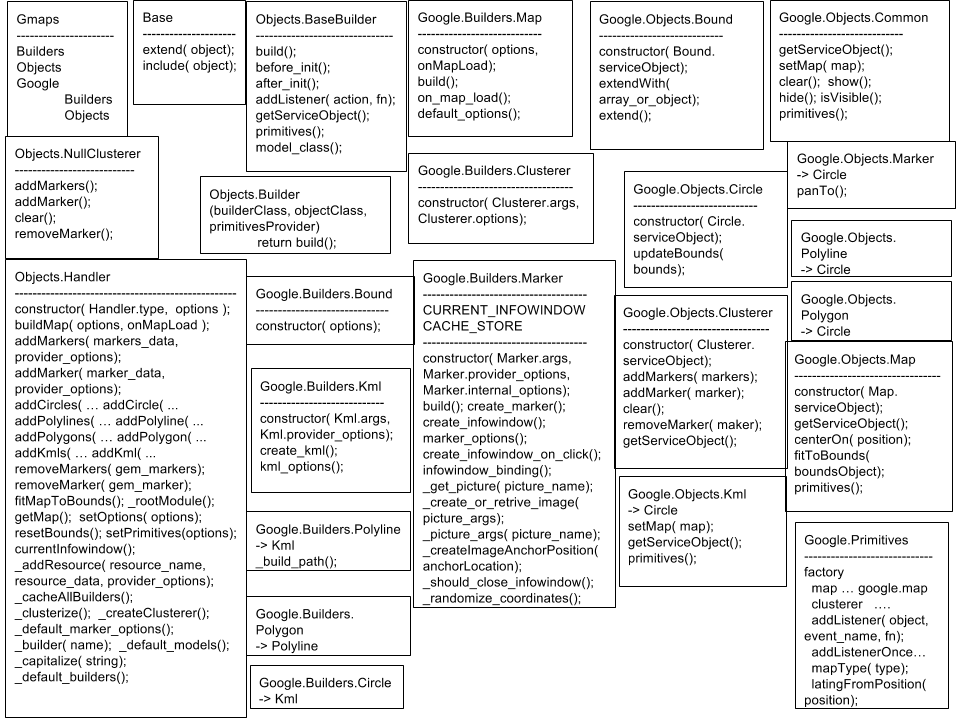
\includegraphics[scale=0.48]{images/diagrama_de_classes_google_maps_for_rails.png}
  \caption{Diagrama de Classes Google-Maps-For-Rails}
  \label{fig:diagrama_de_classes_google_maps_for_rails}
\end{figure}

\begin{comment}
Percebe-se que o diagrama de classe na imagem ‘‘Figure \ref{fig:diagrama_de_classes_google_maps_for_rails} - 
Diagrama de Classes Google-Maps-For-Rails'' não segue os padrões de um diagrama de classes, por causa que 
no espaço disponível na imagem não seria possível inserir o sistema por completo, comprometendo o 
entendimento da gema. Por esse motivo as definições deste diagrama serão explicados logo a seguir.
\end{comment}

As seguintes explicações são válidas para o diagrama de classe na imagem ‘Figure 
\ref{fig:diagrama_de_classes_google_maps_for_rails} - Diagrama de Classes Google-Maps-For-Rails'':

\begin{itemize}

 \item O digrama não mostra os atributos das classes. 
 
 \item Todos os nomes seguidos de ‘‘(...)'' abiaxo do traço ‘‘-----'' representam os métodos da classe.
 
 \item Existem classes que não possuem os traços ‘‘-----'', neste caso elas possuem o nome delas
 seguida do símbolo ‘‘->'' e depois um nome de outra classe. Isso significa que esta classe
 possui os mesmo métodos da classe que vem depois do símbolo ‘‘->''. Por exemplo a 
 classe ‘‘\emph{Google.Builder.Circle -> Kml}'' representa a classe ‘‘\emph{Google.Builder.Circle}'' 
 e ela possuí os mesmo métodos da classe ‘‘\emph{Kml}'', ou seja, ela possuí os métodos
 ‘‘\emph{constructor()}'', ‘‘\emph{create\_...()}'' e ‘‘\emph{...\_option()}''. E também existe o caso 
 onde esta classe possuí métodos além dos da outra, e neesse caso esses métodos são colocados na linha 
 de baixo. Por exemplo a classe ‘‘\emph{Google.Builder.Polyline -> Kml}'' que é a classe 
 ‘‘\emph{Google.Builder.Polyline}'', além de possuír os métodos da classe \emph{Kml}, ela 
 possuí o método ‘‘\emph{\_build\_path()}''.
 
\end{itemize}

\begin{figure}[ht]
  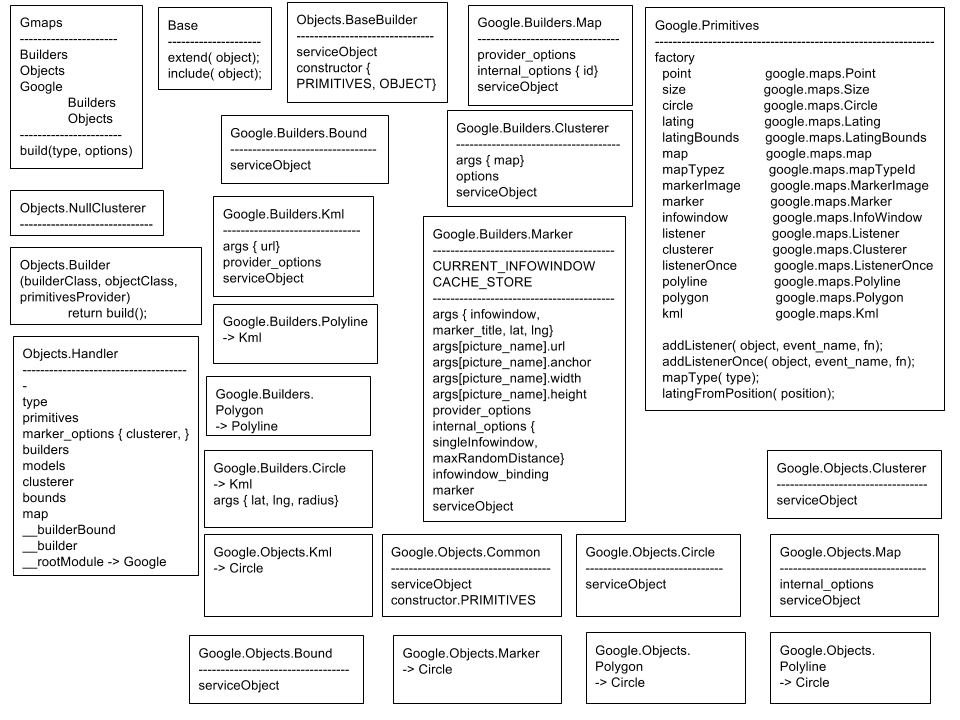
\includegraphics[scale=0.48]{images/diagrama_de_atributos_google_maps_for_rails.png}
  \caption{Diagrama de Atributos Google-Maps-For-Rails}
  \label{fig:diagrama_de_atributos_google_maps_for_rails}
\end{figure}

\begin{comment}
O diagrama de atributos na imagem ‘‘Figure \ref{fig:diagrama_de_atributos_google_maps_for_rails} - 
Diagrama de Atributos Google-Maps-For-Rails'' não é um diagrama padrão de projeto, mas neste caso ele
serve como complemento do diagrama de classe ‘‘Figure \ref{fig:diagrama_de_classes_google_maps_for_rails} - 
Diagrama de Classes Google-Maps-For-Rails'', e isso também foi feito por causa do pouco
espaço disponível na imagem. Por esse motivo as definições deste diagrama serão explicados logo a seguir.
\end{comment}

As seguintes explicações são válidas para o diagrama de de atributos na imagem ‘‘Figure 
\ref{fig:diagrama_de_atributos_google_maps_for_rails} - Diagrama de Atributos Google-Maps-For-Rails'':

\begin{itemize}
 
 \item Todos os nomes abiaxo do traço ‘‘-----'' representam os atributos da classe. Também 
 existe o caso onde esse métodos são seguidos pelos símbolos ‘‘\{ ... \}'', onde o método é um 
 \emph{objeto} e os nomes separados por ‘‘,'' entre os símbolos ‘‘\{ ... \}'' são os atributos
 do \emph{objeto}.
 
 \item Existem classes que não possuem os traços ‘‘-----'', neste caso elas possuem o nome delas
 seguida do símbolo ‘‘->'' e depois um nome de outra classe. Isso significa que esta classe 
 possui os mesmo atributos da classe que vem depois do símbolo ‘‘->''. Por exemplo a 
 classe ‘‘\emph{Google.Builder.Polyline -> Kml}'' que representa a classe 
 ‘‘\emph{Google.Builder.Polyline}'', ela possuí os mesmo atributos da classe
 ‘‘\emph{Kml}'', ou seja, ela possuí os atributos 
 ‘‘\emph{args \{ url \}}'', ‘‘\emph{provider\_option}'' e ‘‘\emph{serviceObject}''. E também existe o caso 
 onde esta classe possuí atributos além dos da outra classe e neesse caso esses 
 atributos são colocados na linha de baixo. Por exemplo a classe 
 ‘‘\emph{Google.Builder.Circle -> Kml}'' que é a classe ‘‘\emph{Google.Builder.Circle}'', além de 
 possuír os atributos da classe \emph{Kml}, ela possuí o atributo 
 ‘‘\emph{args \{ lat, lng, radius \}}''.
 
\end{itemize}

\begin{figure}[ht]
  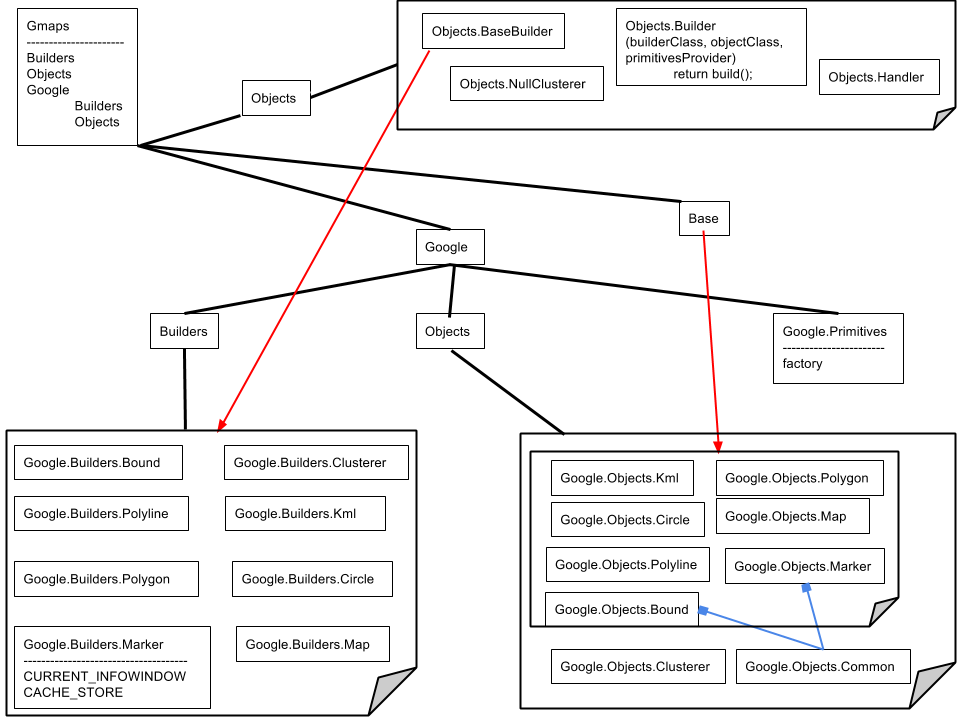
\includegraphics[scale=0.48]{images/diagrama_de_heranca_google_maps_for_rails.png}
  \caption{Diagrama de Herança Google-Maps-For-Rails}
  \label{fig:diagrama_de_heranca_google_maps_for_rails}
\end{figure}

\begin{comment}
O diagrama de herança na imagem ‘‘Figure \ref{fig:diagrama_de_heranca_google_maps_for_rails} - 
Diagrama de Herança Google-Maps-For-Rails'' não é um diagrama padrão de projeto, mas neste caso ele também
serve como complemento do diagrama de classe ‘‘Figure \ref{fig:diagrama_de_classes_google_maps_for_rails} - 
Diagrama de Classes Google-Maps-For-Rails'', e isso também foi feito por causa do pouco
espaço disponível na imagem. Por esse motivo as definições deste diagrama serão explicados logo a seguir.
\end{comment}

As seguintes explicações são válidas para o diagrama de herança na imagem ‘‘Figure 
\ref{fig:diagrama_de_heranca_google_maps_for_rails} - Diagrama de Herança Google-Maps-For-Rails'':

\begin{itemize}

 \item As linhas pretas indicam a organização da gema sendo que a classe \emph{Gmaps} é a classe principal.
 
 \item Os retângulos normais representam as classes.
 
 \item A classe \emph{Gmaps} possui os atributos \emph{Builders}, \emph{Objects} e 
 \emph{Google}, onde o \emph{Google} possui os atributos \emph{Builders} e \emph{Objects}.
 
 \item As linhas vermelhas com pontas de seta representam a herança entre duas \emph{classes}, onde 
 a classe que está com a seta, é a classe que herda as características da classe
 na outra ponta da linha.

 \item As linhas azuis com pontas de quadrado representam a inclusão de uma classe na outra, onde
 a classe que está com o quadrado, é a classe que incluí a classe que está na outra ponta da linha.
 
  \item Os retângulos que tem uma dobra no canto inferior direito representam um conjunto de classes, 
 onde estas classes possuem uma característica em comum. Por exemplo as classes ‘‘\emph{Kml}'', 
 ‘‘\emph{Polygon}'', ‘‘\emph{Polyline}'', ‘‘\emph{Circle}'', ‘‘\emph{Map}'', ‘‘\emph{Marker}'' e 
 ‘‘\emph{Bound}'' que são ‘‘\emph{Objects}'' do ‘‘\emph{Google}'', estão em um conjunto onde todas elas 
 herdam as características da classe ‘‘\emph{Base}''.
 
 \end{itemize}
 
 
\subsection{Entendimento da gema} 
\label{subsection:entendimento_da_gema} 

Agora que realizamos a \emph{engenharia reversa} da \emph{gema}, podemos analisar algumas de suas 
características que serão listadas e explicadas logo a seguir.

\begin{itemize}

 \item Apesar do ‘‘\emph{GMaps}'' ser a classe principal da gema, ela não é a mais
 importante, pois todas as funcionalidades da gema são controladas pela classe
 ‘‘\emph{Hanlder}''. A única funcionalidade da classe ‘‘\emph{GMaps}'' é fazer a chamada
 para a criação de ‘‘\emph{Handler}'', ou seja quando se requisita o método 
 ‘‘\emph{GMaps.build('Google')}'' o método verifica se o objeto ‘‘\emph{Handler}'' já
 existe, e caso ele não exista, o ‘‘\emph{GMaps}'' faz a criação chamando o método 
 ‘‘\emph{new Gmaps.Objects.Handler(type, options)}''.

 \item ‘‘\emph{Hander}'' é a classe que controla todo o funcionamento da gema e 
 basicamente ela possui dois momentos:
 
  \subitem - No primeiro momento ela prepara a estrutura da \emph{gema} para criação e manipulação
  do mapa, criando e setando os objetos de configuração, como por exemplo criando o \emph{objeto}
  ‘‘\emph{Primitives}''.
  
  \subitem - No segundo momento ela cria o mapa com as configurações e permite a manipulação do mapa, 
  possibilitando a criação e inserção de sobreposições como \emph{circles} e \emph{polylines}.
 
 \item A classe ‘‘\emph{Primitives}'' possui as definições que são comuns na gema, 
 como por exemplo, é ela possui a definição do tipo ‘‘\emph{Marker: google.maps.Marker}'' que 
 é a classe \emph{Marker} do \emph{Google Maps}.
 
 \item O atributo ‘‘\emph{serviceObject}'' de todas as classes de 
 ‘‘\emph{Builders}'' do ‘‘\emph{Google}'', representam o atributo que recebe o objeto do 
 \emph{Google Maps}.
 
\end{itemize}
 
\subsection{Adaptações}
\label{subsection:adaptações}

Agora que temos uma abstração de alto nível para a gema \emph{Google-Maps-For-Rails} podemos partir para a 
adaptação dela, ou seja, agora que temos alguns diagramas que nos auxiliam a visualizar o funcionamento 
geral da gema, podemos tentar acrescentar novas funcionalidades, analisando os locais das possíveis 
modificações e os impactos que essas mudanças podem causar. 

A gema já possuí sobreposições como \emph{markers} e \emph{circles}, mas até o momento não possuí a 
funcinalidade de criar direções entre um ponto de origem e um ponto de destino. Contudo a ideia é criar 
uma funcionalidade que receba como parâmetro um local de origem e um local de destino e retorne como
resultado uma sequência de ruas e direções a serem seguidas para ir do local de origem ao local de destino.

Para realizarmos essa modificação foi necessário consultar a \emph{API} do 
\emph{\href{https://developers.google.com/maps/documentation/javascript/directions}{Direction Service}} 
\footnote{Direction Service: \url{https://developers.google.com/maps/documentation/javascript/directions}}
(\emph{Serviço de Direção}) do \emph{Google}, onde verificamos que seria necessário o uso de pelo menos
quatro \emph{classes} que serão listadas e explicadas logo a seguir:

\begin{itemize}

 \item ‘‘\emph{DirectionService}'' (\emph{google.maps.DirectionsService}) que é a classe que tem o 
 objetivo de requisitar e receber o caminho entre o local de origem e o local de destino.
 
 \item ‘‘\emph{DirectionRender}'' (\emph{google.maps.DirectionsRenderer}) que é a classe que tem o 
 objetivo de rederizar no mapa o caminho entre o local de origem e o local de destino.
 
 \item ‘‘\emph{TravelMode}'' (\emph{google.maps.TravelMode}) que é a classe que tem o objetivo de 
 informar a forma como esse caminho deve ser percorrido, que pode ser caminhando (walking), de carro 
 (driving), bicicleta (bicycling) e/ou por meios de locomoção públicos (transit).
 
 \item ‘‘\emph{DirectionsStatus}'' (\emph{google.maps.DirectionsStatus}) que é a classe que tem o
 objetivo de informar o \emph{status} da requisição feita pela objeto da classe
 ‘‘\emph{DirectionService}''.
 
\end{itemize}

Sabendo da necessidade da inclusão de ‘‘\emph{DirectionService}'', ‘‘\emph{DirectionRender}'',
‘‘\emph{TravelMode}'' e ‘‘\emph{DirectionsStatus}'', decidimos que a primeira modificação na gema seria 
incluir estas quatros classe nas definições da classe ‘‘\emph{Primitives}''. E isso foi 
feita da seguinte forma como apresentado no código ‘‘Código 
\ref{lst:classe_primitives_com_atributos_de_directions} - Classe Primitives com atributo de Directions'' 
logo abaixo.

\lstinputlisting[ style=customCoffee, caption={Classe Primitives com atributo de Directions}, label={lst:classe_primitives_com_atributos_de_directions}]
{codigos/classe_primitives_com_atributos_de_directions.coffee}

\begin{figure}[ht]
  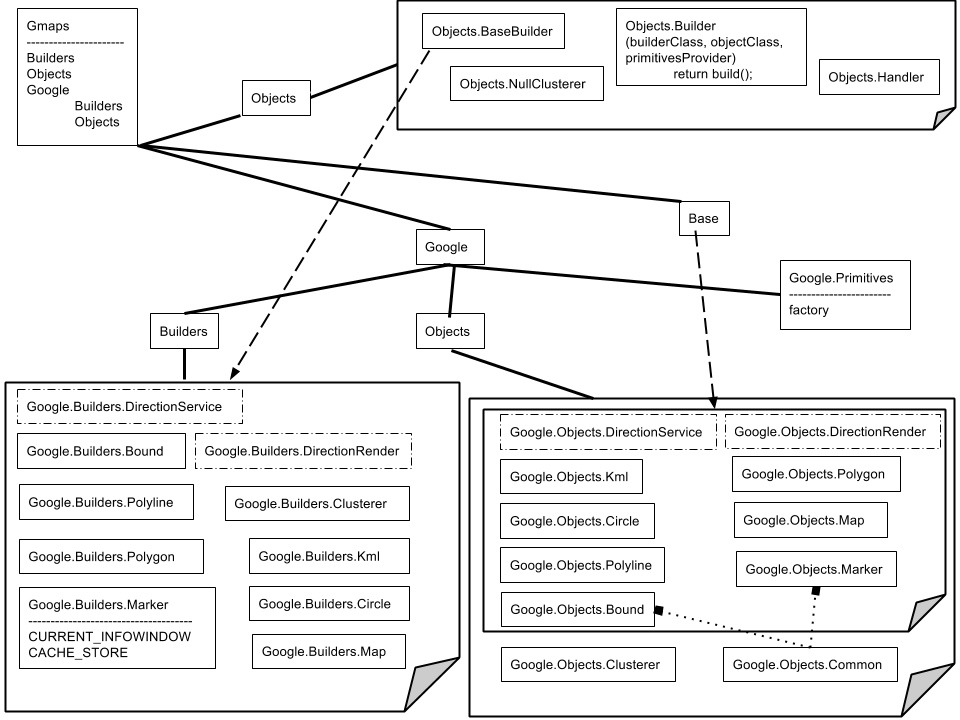
\includegraphics[scale=0.48]{images/novo_diagrama_de_heranca_google_maps_for_rails.png}
  \caption{Novo Diagrama de Herança Google-Maps-For-Rails}
  \label{fig:novo_diagrama_de_heranca_google_maps_for_rails}
\end{figure}

Em seguida criamos quatro \emph{classes} para o ‘‘\emph{Google}'', sendo que duas são ‘‘\emph{Builders}'' de 
‘‘\emph{DirectionService}'' e ‘‘\emph{DirectionRender}'', e as outras duas são ‘‘\emph{Objects}'' também das 
classes ‘‘\emph{DirectionService}'' e ‘‘\emph{DirectionRender}''. Para facilitar a compreensão, elaboramos o 
diagrama representado na imagem ‘‘Figure \ref{fig:novo_diagrama_de_heranca_google_maps_for_rails} - Novo 
Diagrama de HrançaGoogle-Maps-For-Rails'' para mostrar o local aonde inserimos as classes e quais as 
dependências que elas possuem. No caso este diagrama é o mesmo diagrama de herança que desenvolvemos na 
\emph{engenharia reversa}, mostrado na imagem ‘‘Figure \ref{fig:diagrama_de_heranca_google_maps_for_rails} - 
Diagrama de Herança Google-Maps-For-Rails'', com a adição das quatro classes que são representadas 
por retângulos tracejados.

Agora que acrescentamos estas quatro classes na gema adaptada, devemos adicionar no ‘‘\emph{Handler}'', 
novas funções para maminpular essas classes. E neste caso inserimos as funçãoes ‘‘\emph{addDirection()}'' e 
‘‘\emph{calculate\_route()}'' que podem ser vistas no código ‘‘Código 
\ref{lst:funcoes_adicionais_do_handler} - Funções adicionais do Handler'' que será explicado logo a seguir.

\begin{itemize}

 \item Na linha ‘‘2'' é adicionado a função ‘‘\emph{addDirection}'' que recebe como parâmetro 
 ‘‘\emph{direction\_data}'', que possui o informações do local de origem e local de destino que são 
 obrigatórios para criar a direção, e ‘‘\emph{provider\_options}'' que pode conter as opções da forma
 como esse direção deve ser gerada. Essa função tem por objetivo criar as direções e colocá-las no mapas.
 
 \item Na linha ‘‘13'' é adicionado a função ‘‘\emph{calculate\_route}'' com o parâmetro 
 ‘‘\emph{direction\_data}'' que tem por principal objtivo fazer a requisição para o \emph{Google } de uma 
 possível direção entre o local de origem ao local de destino.
 
 \item Da linha ‘‘3'' a linha ‘‘10'' é o conteúdo da função ‘‘\emph{addDirection}'', onde se cria os
 atributos ‘‘\emph{direction\_service}'' e ‘‘\emph{direction\_render}'' para o ‘‘\emph{Handler}'', e
 para cada um deles é atribuido o seu respectivo objeto do \emph{Google Maps} com a chamada da função 
 ‘‘\emph{@\_builder(...)}''. Depois é feito a chamada da função ‘‘\emph{calulate\_route(...)}''
 para encontrar uma possível direção e finalmente com o código 
 ‘‘\emph{@direction\_render.getServiceObject().setMap(@getMap())}'' a direção encontrada é colocado 
 no mapa.
 
 \item Da linha ‘‘13'' a linha ‘‘20'' é o conteúdo da função ‘‘\emph{calculate\_route(...)}'', onde 
 inicialmente é colocado em uma variável local o \emph{status Ok} de requisição que será utilizado
 para verificar se a requisição de direção foi feita com sucesso, e também é criada uma variável local 
 para o \emph{objeto DirectionRender} do \emph{Google Maps}. Em seguida através da chamada da função 
 ‘‘\emph{route(...)}'' do \emph{objeto DirectionService} que passa como parâmetro o local de origem e
 o local de destino e recebe como resposta o \emph{status} da requisição e o \emph{response} que pode
 conter o caminho solução. Após a execução desta função é feita a verificação da resposta, e caso 
 ela venha como o \emph{status Ok} o \emph{objeto DirectionRender} recebe o caminho solução.
 
\end{itemize}

\lstinputlisting[ style=customCoffee, caption={Funções adicionais do Handler}, label={lst:funcoes_adicionais_do_handler}]
{codigos/funcoes_adicionais_do_handler.coffee}

\subsection{Exemplo de uso de Google-Maps-for-Rails}
\label{subsection:exemplo_de_uso_de_google-maps-for-rails}

Como exemplo de uso da gema ‘‘\emph{Google-Maps-for-Rails}'' adaptada criamos o projeto 
‘‘\emph{\href{https://github.com/toshikomura/DiseasesMap}{DiseasesMap}}'' 
\footnote{DiseasesMap : \url{https://github.com/toshikomura/DiseasesMap}} que tem como objetivo representar 
a frequência de doenças no mapa do \emph{Google} utilizando sobreposições. Até o momento de término deste
trabalho essa função ainda não havia sido implementada, mas fizemos o uso da funcionalidade de direções.

Inicialmente fizemos a instalção e inclusão da gema adaptada no arquivo \emph{Gemfile} do projeto. Depois 
criamos uma estrutura básica de \emph{model/view/controller} de ‘‘\emph{locations}''. 

Em seguida para fazer o uso da função de direções utilizamos o código‘‘Código 
\ref{lst:exemplo_coffeescript_que_cria_mapa_com_direcao} - Exemplo CoffeeScript que Cria Mapa com 
Direção'' explicado logo abaixo.

\lstinputlisting[ style=customCoffee, caption={Exemplo CoffeeScript que Cria Mapa com Direção}, label={lst:exemplo_coffeescript_que_cria_mapa_com_direcao}]
{codigos/DiseasesMap/app/assets/javascripts/locations.js.coffee}

\begin{itemize}

 \item Na linha ‘‘6'' é feita a preparação da estrtura de configuração do mapa com a chamada 
 ‘‘\emph{GMaps.build('Google')}'', sendo feita a criação do \emph{objeto Handler}, que é atribuida a 
 variável local ‘‘\emph{handler}'', juntamente com as outras configurações básicas que o mapa necessita.
 
 \item Na linha ‘‘7'' é feita a chamada de ‘‘\emph{handler.buildMap(...)}'' que tem como função fazer a 
 criação do mapa a parir das configurações básicas já definidas quando foi feita a chamada de 
 ‘‘\emph{GMaps.build('Google')}''. São passados como parâmetros as variáveis, ‘‘\emph{provider}''
 que neste caso está vazio, e internal que define o ‘‘\emph{id}'' do mapa como ‘‘\emph{map}'', neste caso
 o ‘‘\emph{id}'' serve para identificar o mapa a ser modificado.
 
 \item Na linha ‘‘11'' é criado uma \emph{function} determinada pelo símbolo ‘‘->'', onde ela somente será 
 executada depois que a função ‘‘\emph{handler.buildMap(...)}'' terminar, ou seja, quando toda a criação do mapa for 
 concluída. Neste caso essa função executa as seguintes operações:
 
  \subitem Na linha ‘‘12'' é feita a criação de um \emph{marker} com a chamada da função 
  ‘‘\emph{handler.addMarker(...)}'', sendo passado como parâmetro, a sua posição que no caso é (0,0) 
  definido ‘‘\emph{lat}'' e ‘‘\emph{lng}'', a sua imagem definida por ‘‘\emph{picture}'', e sua informação 
  definido por ‘‘\emph{infowindow}''.
 
  \subitem Na linha ‘‘22'' é feita a extensão de fronteiras incluindo o novo \emph{marker} com a chamada 
  da função ‘‘\emph{handler.bounds.extendWith(...)}'', sendo passado como parâmetro o \emph{marker} criado
  anteriormente.
 
  \subitem Na linha ‘‘23'' é feita a criação de direções com a chamada da função 
  ‘‘\emph{handler.addDirection(...)}''que incluimos no ‘‘\emph{Handler}'', sendo passado como parâmetro, um 
  local de origem definido por ‘‘\emph{ origin: ‘‘São Paulo''} '', e um local de destino definido por 
  ‘‘\emph{destination: ‘‘Curitiba''} ''.
 
\end{itemize}

E para mostrar o mapa na view de ‘‘\emph{locations}'' adicionamos o código mostrado em ‘‘Código 
\ref{lst:exemplo_locations_view_que_cria_mapa_com_direcao} - Exemplo Locations view que Cria Mapa com Direção'' 
que é parte do código da \emph{view}, explicado logo a seguir.

\lstinputlisting[ style=customRubyHTML, caption={Exemplo Locations view que Cria Mapa com Direção}, label={lst:exemplo_locations_view_que_cria_mapa_com_direcao}]
{codigos/index_simplificado.html.erb}

\begin{itemize}

 \item Na linha ‘‘1'' com a \emph{tag} \emph{<h1>...</h1>} é definido como título principal da \emph{view} o
 texto ‘‘\emph{Listining locations}''.
 
 \item Os ‘‘\emph{...}'' indica que existe código, mas por simplificação na explicação, ele não fo mostrado.
 
 \item Da linha ‘‘3'' a ‘‘5'' é definido uma \emph{div} com ‘‘800px'' de largura, e dentro dessa \emph{div}
 é definido o local para a criação do mapa com ‘‘800px'' de largura e ‘‘400px'' de altura. No caso o local 
 de criação do mapa é referênciado pelo atributo \emph{id} que o mesmo \emph{id} utilizado no código 
 ‘‘Código \ref{lst:exemplo_coffeescript_que_cria_mapa_com_direcao} - Exemplo CoffeeScript que Cria Mapa com 
 Direção'' na linha ‘‘10''.  
 
\end{itemize}

Como resultado ao se acessar o \emph{index} de locations obtemos como resultado a imagem ‘‘Figure 
\ref{fig:caminho_entre_sao_paulo_e_curitiba} - Caminho entre São Paulo e Curitiba''. Neste caso a
nossa gema adaptada com a nova funcionalidade de direções funcionou corretamente, pois o caminho
mostrado é entre ‘‘São Paulo'' e ‘‘Curitiba'' como requisitamos na linha ‘‘24'' do código ‘‘Código 
\ref{lst:exemplo_coffeescript_que_cria_mapa_com_direcao} - Exemplo CoffeeScript que Cria Mapa com Direção''.

 \begin{figure}[ht]
  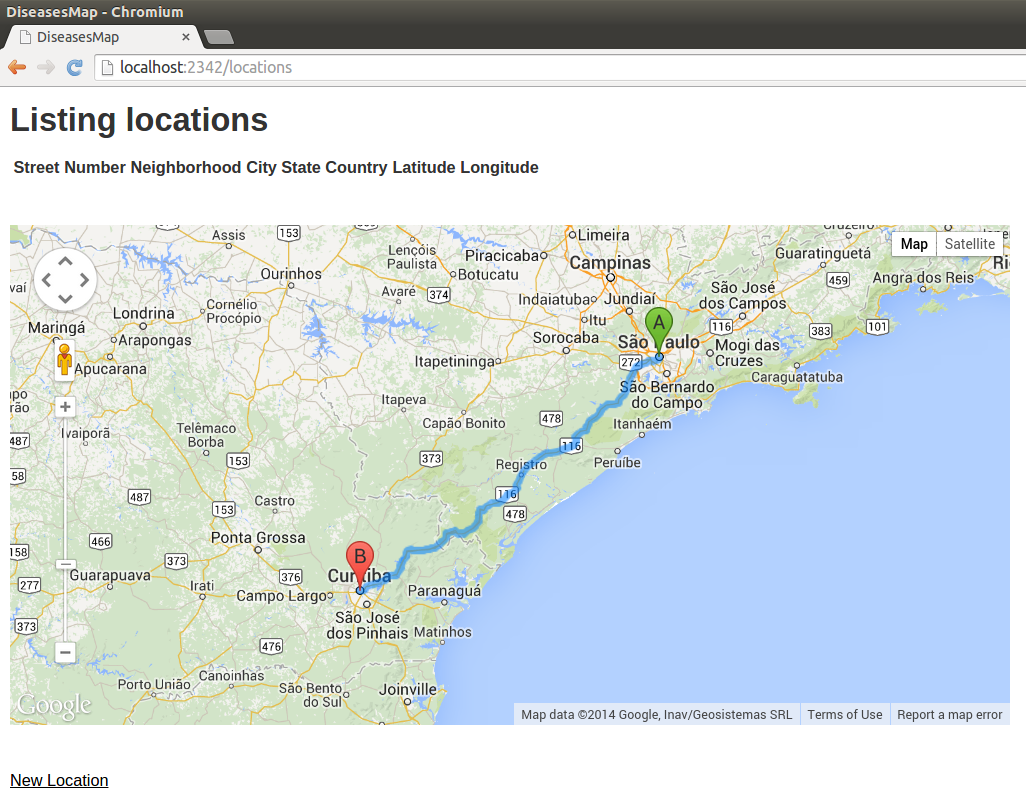
\includegraphics[scale=0.44]{images/caminho_entre_sao_paulo_e_curitiba.png}
  \caption{Caminho entre São Paulo e Curitiba}
  \label{fig:caminho_entre_sao_paulo_e_curitiba}
\end{figure}

% ---
% Finaliza a parte no bookmark do PDF, para que se inicie o bookmark na raiz
% ---
\bookmarksetup{startatroot}% 
% ---

% ----------------------------------------------------------
% Conclusão
% ----------------------------------------------------------
\chapter[Conclusão]{Conclusão}
\label{chapter:conclusao}
\begin{frame}
\frametitle{Trabalhos Futuros}
 
  \begin{block}{Trabalhos Futuros}
   
   \begin{itemize}
   
    \item Para a primeira gema de exemplo \emph{\textbf{gemtranslatetoenglish}}:
    
    \begin{itemize}
    
     \item Abordar mais recursos da linguagem \emph{\textbf{Ruby}}.
     
     \item Desenvolver mais funcionalidades para mostrar mais modelos de teste.
     
    \end{itemize}

    \item Para a segunda gema de exemplo \emph{\textbf{Google-Maps-For-Rails adaptada}}:
    
    \begin{itemize}
    
     \item Incluir a escolha de locomoção.
     
     \item Incluir a possibilidade de inserir pontos intermediários entre a origem e o destino.
     
    \end{itemize}

    
   \end{itemize}
   
  \end{block}
 
\end{frame}


\begin{frame}
 \frametitle{Conclusão}

  \begin{block}{Conclusão}
   
   \begin{itemize}
   
    \item Proporcionou o entendimento sobre bibliotecas.
    
    \item Mostrou conceitos básicos da linguagem \emph{\textbf{Ruby}}.
    
    \item Apresentou como criar uma biblioteca do \emph{\textbf{Ruby}}.
    
    \item Mostrou como adaptar uma biblioteca do \emph{\textbf{Ruby}}.
    
    \item Apresentou exemplos para facilitar o entendimento da explicação de como criar ou adaptar uma
    biblioteca do \emph{\textbf{Ruby}}.
    
    \item Proporcionou a possibilidade de economizar tempo no desenvolvimento.
    
   \end{itemize}      
   
  \end{block}
  
\end{frame}  

% ----------------------------------------------------------
% ELEMENTOS PÓS-TEXTUAIS
% ----------------------------------------------------------
\postextual

% ----------------------------------------------------------
% Referências bibliográficas
% ----------------------------------------------------------
\bibliography{referencias}

% ----------------------------------------------------------
% Apêndices
% ----------------------------------------------------------
\begin{apendicesenv}

\partapendices

\chapter[Classificação de Bibliotecas]{Classificação de Bibliotecas}
\label{chapter:classificação_de_bibliotecas}
As bibliotecas podem ser indentificadas pelo seu tipo de classificação, onde as suas classificações
podem ser definidas pela maneira como elas são ligadas que é explicado na sub-seção
\ref{section:formas_de_ligamento}, pelo momento que elas são ligadas que é explicado na sub-seção
\ref{section:momentos_de_ligação}, e pela forma como elas são compartilhadas que é explicado na
sub-seção \ref{section:formas_de_compartilhamento}.

\section{Formas de ligamento}
\label{section:formas_de_ligamento}

O processo de ligamento implica em associar uma biblioteca a um programa ou outra biblioteca, ou seja,
é nesse momento que as implementações das funcionalidades são realmentes ligadas ao programa ou
outra biblioteca.

Esse processo de ligamento pode ser feito de 3 formas diferentes:

\begin{itemize}

 \item \emph{\textbf{Tradicional}} que significa que os dados da biblioteca são copiados para o executável do programa
 ou outra biblioteca.

 \item \emph{\textbf{Dinâmica}} que significa que ao invés de copiar os dados da biblioteca para o executável, é
 somente feito uma referência do arquivo da biblioteca. Neste caso o ligador não tem tanto
 trabalho na compilação, pois ele somente grava a biblioteca a ser utilizada e um indice para
 ela, passando todo o trabalho para o momento onde a aplicação é carregada para a memória ou para
 o momento que a aplicação requisita a biblioteca.

 \item \emph{\textbf{Remoto}} que significa que a biblioteca vai ser carregada por chamadas de procedimento remotos,
 ou seja, a biblioteca pode ser carregada mesmo não estando na mesma máquina do programa ou
 biblioteca, pois ela é carregada pela rede.

\end{itemize}

\section{Momentos de ligação}
\label{section:momentos_de_ligação}

O momento de ligação diz respeito ao momento em que a biblioteca vai ser carregada na memória e
para esse caso existem 2 formas:

\begin{itemize}

 \item \emph{\textbf{Carregamento em tempo de carregamento}} que significa que a biblioteca vai ser
 carregada na memória quando a aplicação também estiver sendo carregada.

 \item \emph{\textbf{Carregamento dinâmico ou atrasado}} que signfica que a biblioteca só vai ser carregada na
 memória quando a aplicação requisitar o seu carregamento e isso é feito em tempo de execução.

\end{itemize}

\section{Formas de compartilhamento}
\label{section:formas_de_compartilhamento}

As formas de compartilhamento de bibliotecas se divide em 2 conceitos. Sendo que o primeiro se refere
ao compartilhamento de código em disco entre os vários programas. E o segundo se refere ao
compartilhamento da biblioteca na memória em tempo de execução.

O compartilhamento em mémória traz a vantagem de que dois ou mais programas podem
compartilhar o acesso ao mesmo código da biblioteca na memória, com isso se evita que a mesma
biblioteca seja colocada mais de uma vez na memória.

Por exemplo para o segundo conceito, suponha que os programas \emph{P1} e \emph{P2} necessitem de
uma biblioteca \emph{B} que é carregada no \emph{momento de carregamento}. Suponha
agora que executamos o programa \emph{P1} e depois de um tempo executamos o programa \emph{P2}, desta
forma primeiramente o programa \emph{P1} e a biblioteca \emph{B} são carregadas na memória. Como
também executamos o programa \emph{P2}, ele também é carregado na memória, mas sem a necessidade de
carregar a biblioteca \emph{B}, pois ela já havia sido carregada anteriomente.

Pensando pelo outro lado, o compartilhamento de memória pode ser um pouco prejudicial
ao desempenho, pois essa biblioteca deve ser escrita para executar em um ambiente \emph{multi-tarefa}
e isso pode causar alguns atrasos.


\chapter[Ferramentas utilizadas]{Ferramentas utilizadas}
\label{chapter:ferramentas_utilizadas}
Este capítulo tem o objetivo de apresentar as ferramentas que foram utilizadas no tutorial. Na seção
\ref{section:vmware_player}, apresentaremos a ferramenta \emph{VMware® Player}, em seguida na seção
\ref{section:rvm}, apresentaremos a ferramenta \emph{RVM}, depois na seção \ref{section:ruby_on_rails},
apresentaremos o \emph{framework Ruby On Rails}, e por fim na seção \ref{section:git}, apresentaremos
a ferramenta \emph{git}.

\section{VMware® Player}
\label{section:vmware_player}

\emph{\href{http://www.vmware.com/products/player}{VMware® Player}} é um aplicativo de virtualização de 
\emph{desktop} que pode rodar um ou mais sistemas operacionais ao mesmo tempo no mesmo computador sem 
a necessidade de reiniciar a máquina. Possui uma interface fácil de usar, suporte a vários sistemas 
operacionais, como por exemplo \emph{Windows}, \emph{MAC} e \emph{Linux} e é portável 
[\citeonline{vmplayer}].

Com o \emph{VMware® Player} pode-se fazer o compartilhamento de vários recursos, como por exemplo pode-se 
fazer a transferência de arquivos do sistema opercional virtual com o sistema opercional que está rodando 
na máquina fisica. 

\section{RVM}
\label{section:rvm}

\emph{\href{http://rvm.io/}{Ruby Version Manager}} \footnote{RVM: \url{http://rvm.io/}} é uma 
ferramenta de linha de comando que permite facilmente instalar, gerenciar e trabalhar com multiplos ambientes 
do \emph{Ruby} para interpretar um certo conjunto de gemas [\citeonline{rvm}].

 \href{https://github.com/wayneeseguin}{Wayne E. Seguin} \footnote{Wayne E. Seguin: 
 \url{https://github.com/wayneeseguin}} iniciou o projeto do \emph{RVM} em outubro de 2007
e a partir de então com uma considerável experiência programando em \emph{Bash}, \emph{Ruby} e outras 
linguagens obteve o conhecimento suficiente para criar o gerenciador [\citeonline{about_rvm}].

\section{Ruby On Rails}
\label{section:ruby_on_rails}

\emph{\href{http://rubyonrails.org/}{Ruby On Rails}} \footnote{Ruby On Rails: \url{http://rubyonrails.org/}} 
é um \emph{web framework} de código aberto que tem por finalidade facilitar a programação
visando a produtividade sustentável. Este \emph{framework} permite escrever códigos bem estruturados
favorecendo a manutenção de aplicações [\citeonline{ruby_on_rails}].

O \emph{Rails} foi criado em 2003 por \emph{\href{http://david.heinemeierhansson.com/}{David Heinemeier Hansson}}
\footnote{David Heinemeier Hansson: \url{http://david.heinemeierhansson.com/}} e desde então é extendido 
pela equipe do \emph{\href{http://rubyonrails.org/core/}{Rails Core Team}} 
\footnote{Rails Core Team: \url{http://rubyonrails.org/core/}} e mais de 3.400 usuários 
[\citeonline{ruby_on_rails}].

\section{Git}
\label{section:git}

\emph{\href{http://git-scm.com/}{Git}} \footnote{Git: \url{http://git-scm.com/}} é um sistema distribuído de 
controle de versão livre e de código aberto, desenhado para controlar projetos pequenos e grandes com 
rapidez e eficiência. É uma ferramenta fácil de manipular com alto desempenho [\citeonline{git}].

Por irônia do destino o \emph{git} foi criado em 2005 por 
\emph{\href{http://torvalds-family.blogspot.com.br/}{Linus Torvalds}} 
\footnote{Linus Torvalds: \url{http://torvalds-family.blogspot.com.br/}} graças ao fim da relação entre a 
comunidade que desenvolvia o \emph{Linux} e a compania que desenvolvia o 
\emph{\href{http://www.bitkeeper.com/}{BitKeeper}}, ferramenta que até aquele ano fazia o gerênciamento de 
código do \emph{Linux}. Sem uma ferramento \emph{SCM} (\emph{Source Code Management}), \emph{Torvalds} 
resolveu desenvolver uma ferramenta parecida com o \emph{BitKeeper} que possuiria mais velocidade,
\emph{design} simples, grande suporte para \emph{non-linear development} (centenas de \emph{branchs}), 
completamente distribuído e capacidade de controlar grandes projeto com grandes quantidades de dados.

\chapter[Preparação do ambiente]{Preparação do ambiente}
\label{chapterss:preparação_do_ambiente}
Para seguir com este trabalho, será necessário a instalação de alguns softwares para que se possa realizar
o passo-a-passo de como criar ou adaptar uma \emph{gema} do \emph{Ruby}.
Inicialmente por comodidade utilizaremos o sistema operacional 
\emph{\href{http://releases.ubuntu.com/12.04/}{Ubuntu 12.04 LTS}}, pois a comunidade prometeu manter essa 
versão por pelo menos 5 anos, com o 
\emph{\href{https://www.ruby-lang.org/en/downloads/}{Ruby 1.9.3p547 (2014-05-14 revision 45962) [i686-linux]}} 
que era a versão mais recente do \emph{Ruby} no momento de inicio desse trabalho, e o 
\emph{\href{http://rubyonrails.org/download/}{Rails 3.2.12}} que era uma versão que já tinhamos experiência
trabalhando no projeto \emph{\href{http://agendador.c3sl.ufpr.br/}{Agendador}}.

Primeiramente deve-se instalar o \emph{Ubuntu 12.04} no 
\emph{\href{https://my.vmware.com/web/vmware/free\#desktop_end_user_computing/vmware_player/}{VMware® Player}}, 
e no nosso caso foi utilizado o \emph{VMware Player 6.0.3 build-1895310}. Após a instalação do \emph{Ubuntu}
deve-se logar no \emph{Ubuntu}, acessar um \emph{terminal}, e fazer a isntalação do 
\emph{\href{https://github.com/wayneeseguin/rvm}{RVM 1.25.28}} com os seguinte comandos no código 
\ref{lst:instala_rvm} que serão explicados logo a seguir:
 
 \lstinputlisting[ style=customBash, caption={Instala RVM}, label={lst:instala_rvm}]
 {codigos/install_rvm.sh}
 
\begin{itemize}

\item O comando ‘‘\emph{sudo -i}'' na linha ‘‘2'' é necessário para acessar o usuário root, pois 
  para instalar os outros \emph{softwares} é preciso ser um administrador do sistema.
  
  \item O comando ‘‘\emph{apt-get install curl}'' na linha ‘‘6'' é necessário pois o script de 
  instalação do \emph{RVM} depende do \emph{curl} para executar corretamente.
  
  \item O comando ‘‘\emph{wget https://raw.github.com/wayneeseguin/rvm/master/binscripts/rvm-installer}'' 
  na linha ‘‘9'' é necessário para baixar o script (‘‘\emph{rvm-installer}'') de instalação do \emph{RVM}.
  
  \item O comando ‘‘\emph{bash rvm-installer}'' na linha ‘‘12'' é necessário para instalar o \emph{RVM}.
  
\end{itemize}

Ao terminar de instalar o \emph{RVM} deve-se fazer a instalação do \emph{Ruby} que pode ser feita com a 
sequência de comandos do código \ref{lst:instala_ruby}, onde cada comando será 
explicado logo em seguida:
 
\lstinputlisting[ style=customBash, caption={Instala Ruby}, label={lst:instala_ruby}]{codigos/install_ruby.sh}
 
\begin{itemize}

 \item O comando ‘‘\emph{ource "/usr/local/rvm/scripts/rvm"}'' serve para carregar o código do \emph{RVM}.
 
 \item O comando ‘‘\emph{rvm requirements}'' serve para instalar as dependências do \emph{RVM} caso elas 
 ainda não estejam instaladas.
 
 \item O comando ‘‘\emph{rvm install 1.9.3}'' serve para fazer a instalação do \emph{Ruby} versão 1.9.3.
 
 \item O comando ‘‘\emph{rvm --default use 1.9.3}'' serve para informar o \emph{RVM} para usar o \emph{Ruby}
 1.9.3 como default. Essa é uma medida preventiva, pois podem existir outras versões do \emph{Ruby} instaldas.
 
 \item O comando ‘‘\emph{rvm use 1.9.3}'' serve para informar o \emph{RVM} para usar o \emph{Ruby} 1.9.3.
 
\end{itemize}

  
Tammbém pode-se configurar as variáveis de ambiente do \emph{RVM} para não precisar a todo momento executar
o comando ‘‘ source "/usr/local/rvm/scripts/rvm" '', e isso pode ser feito executando o seguinte código
\ref{lst:configura_variavel_rvm} que é exibilido e explicado logo abaixo:
 
\lstinputlisting[ style=customBash, caption={Configura Variáveis RVM}, label={lst:configura_variavel_rvm}]
{codigos/configura_variavel_rvm.sh}
 
\begin{itemize}

  \item O comando ‘‘\emph{echo '...' >> $\sim$/.bashrc }'' pega todo o código, aqui representado por ‘‘...'' 
  e insere no final do arquivo ‘‘$\sim$/.bashrc''. Uma alternativa seria somente copiar o código dentro do 
  ‘‘\emph{echo}'' e colar no final do arquivo ‘‘$\sim$/.bashrc''.
  
\end{itemize}

E depois da execução de todas essa instalações, ainda devemos instalar as gemas essências, ‘‘\emph{rails}'' 
e ‘‘\emph{bundle}'', executando os seguintes comandos no código 
\ref{lst:install_essentials_gems} explicado logo a seguir:
 
\lstinputlisting[ style=customBash, caption={Instala Gemas Essênciais}, label={lst:install_essentials_gems}]
{codigos/install_essentials_gems.sh}

\begin{itemize}

 \item O comando ‘‘ \emph{gem install rails --version ‘3.2.12'} '' faz a instalação da gema \emph{rails}
 versão \emph{3.2.12}.
 
 \item O comando ‘‘\emph{gem install bundle}'' faz a instalação da gema \emph{bundle}.
 
\end{itemize}

\end{apendicesenv}


\end{document}